This section discusses all the architectural decisions taken for building the Students \& Companies (S\&C). In the overview sub-section, the overall architecture of the system is presented along with a diagram which differentiates the architectural layers within the system. Then component view of the software is presented with all the important components and the relationship between all the components are clearly defined. Then in the deployment view decisions related to the deployment of the software is articulated. The flow of interactions between actors and components are shown using sequence diagrams in the Runtime View section. \\

\subsection{Overview: High-level components and their interaction}
The figure below is gives a high-level description of the S\&C system. The different users of system interacts with the client side of our web application which is called the front-end of our application and is in the Application Layer. The back-end comprises of the business logic layers which is used for carrying out all the server applications. Lastly, the data layer which is used for storage and retrieval of the data.

\begin{figure}[H]
\centering
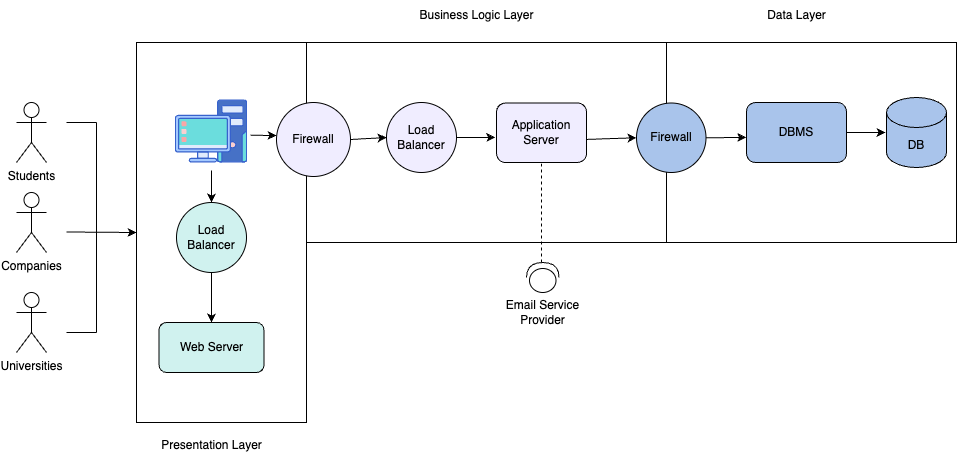
\includegraphics[width=0.8\textwidth]{Images/overview-component.png}
\caption{\label{fig:metamodel4}Presentation Layer, Business Logic Layer and Data Layer}
\end{figure}

\subsection{Component View}
In this section we show the components of the S\&C and their relationships. 

\textbf{Subsystems:}
\begin{enumerate}
    \item \textbf{User Interfaces:}
    \begin{itemize}
        \item \textbf{Student Portal, Company Portal, University Admin Portal:} Interfaces for respective users to interact with the system.
    \end{itemize}

    \item \textbf{Core Systems:}
    \begin{itemize}
        \item \textbf{Recommendation Engine:} Matches students and internships based on data.
        \item \textbf{Feedback and Analytics Module:} Improves recommendations using feedback.
        \item \textbf{Notification Service:} Sends messages/alerts to users.
        \item \textbf{Selection Management System:} Manages interviews and selection processes.
        \item \textbf{Monitoring and Complaints Module:} Tracks internships and manages complaints.
        \item \textbf{Security and Access Control:} Ensures authentication and secure access.
    \end{itemize}

    \item \textbf{Data Storage:}
    \begin{itemize}
        \item \textbf{Database:} Stores CVs, internship details, feedback, and complaints.
    \end{itemize}
\end{enumerate}

\textbf{Connection Types:}
\begin{itemize}
    \item \textbf{\texttt{--( Required Interface:}} Indicates a component requests services (e.g., portals requesting recommendations).
    \item \textbf{\texttt{-(0- Message Interface:}} Represents communication or event-driven messaging (e.g., notifications).
    \item \textbf{\texttt{-0)- Service Interface:}} Represents a request-response model (e.g., selection processes).
    \item \textbf{\texttt{..> Dependency:}} Highlights one component's dependency on another (e.g., feedback improving recommendations).
\end{itemize}

\begin{figure}[H]
\centering
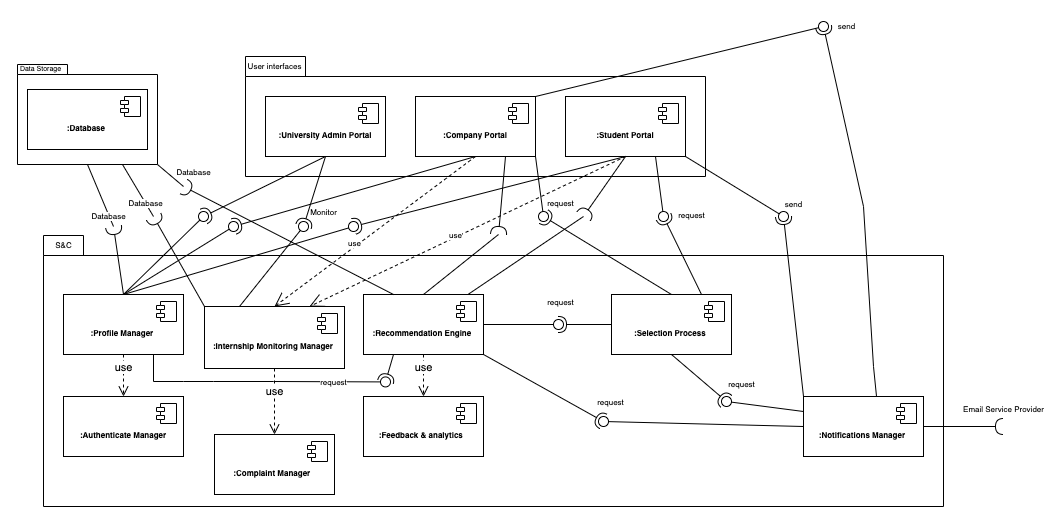
\includegraphics[width=0.8\textwidth]{Images/Component view Diagram.png}
\caption{\label{fig:metamodel4}UML Diagram for Students \& Companies System}
\end{figure}

\subsection{Deployment View}
The S\&C web application is deployed in cloud and uses the benefits that are offered by cloud deployment compared to traditional deployments which will be discussed later.

Client device and access the S\&C web page using any browser of choice. The web pages are loaded from the web server in cloud using HTTP calls. Firewall is used to provide security and allow trusted requests. Elastic load balancer is used to evenly distribute incoming traffic in web servers and application servers. Lastly, the required data are stored in the DB. A standby DB is also added to provide with data connection in case of failure of the main DB. \\ \\

\textbf{Advantages of Cloud - }
\begin{itemize}
\item \textbf{Scalability and Flexibility:} Cloud platforms provide the ability to scale resources up or down quickly based on demand. This is especially useful for businesses with fluctuating needs or growth. Cloud systems automatically scale resources to meet workload changes without manual intervention, optimizing resource utilization.
\item \textbf{Cost Efficiency:} Cloud services offers a pay-per-usage, thus paying only for the resources actually used. Cloud services offer reduced maintenance cost and low infrastructure costs.
\item \textbf{High Availability and Reliability:} Cloud providers usually have data centers in multiple locations, offering built-in redundancy. This ensures high availability and reduces the risk of system outages.
\end{itemize}


\begin{figure}[H]
\centering
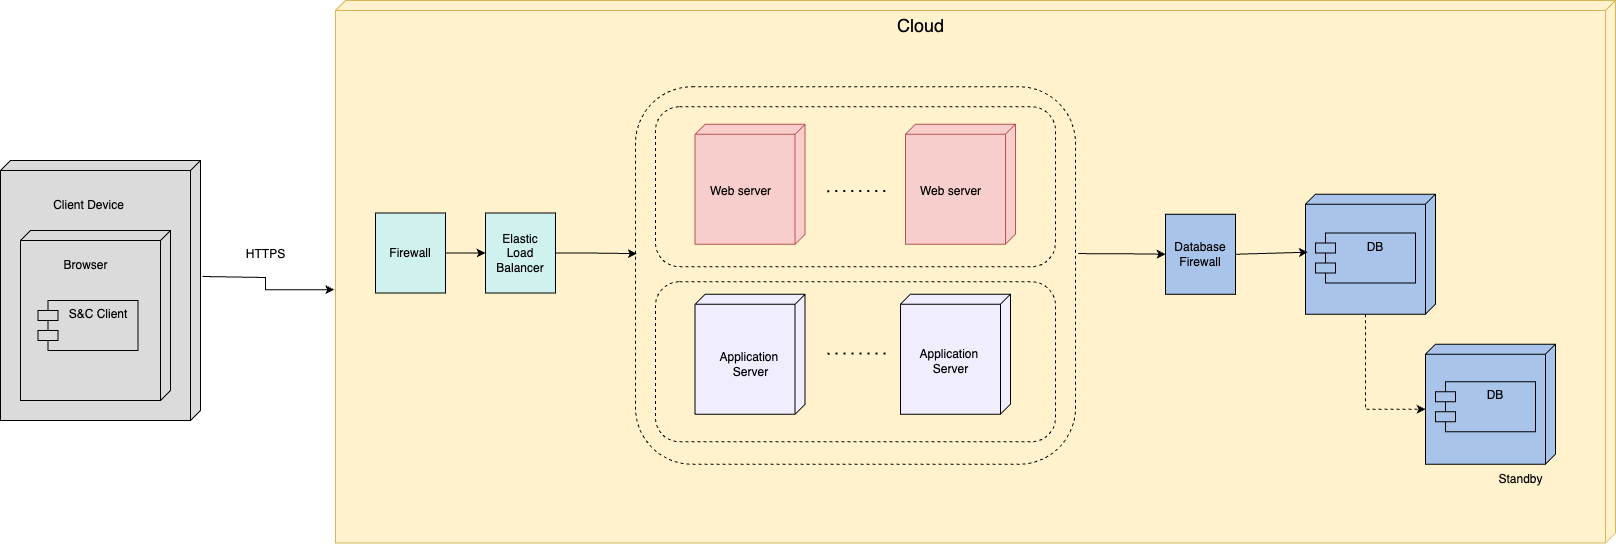
\includegraphics[width=0.8\textwidth]{Images/deployment-view1.png}
\caption{\label{fig:metamodel4}Deployment Diagram}
\end{figure}

\subsection{Runtime View}

\begin{itemize}
    \item \textbf{User Sign Up} \\ \\
    The following diagram is the sequence diagram for the User Sign Up use case depicting all the components engaged for the stated use case. First the User goes to website of S\&C in the browser and tries to Sign Up by giving all the required details. Using API calls the details of the user is sent to the Profile Manager component in the webs server. Profile Manager then sends the data to Entity Manager which connects the database to our server. Then finally data is added to the database. If saving of data is unsuccessful error message is shown to the user else success message is shown.
    \begin{figure}[H]
    \centering
    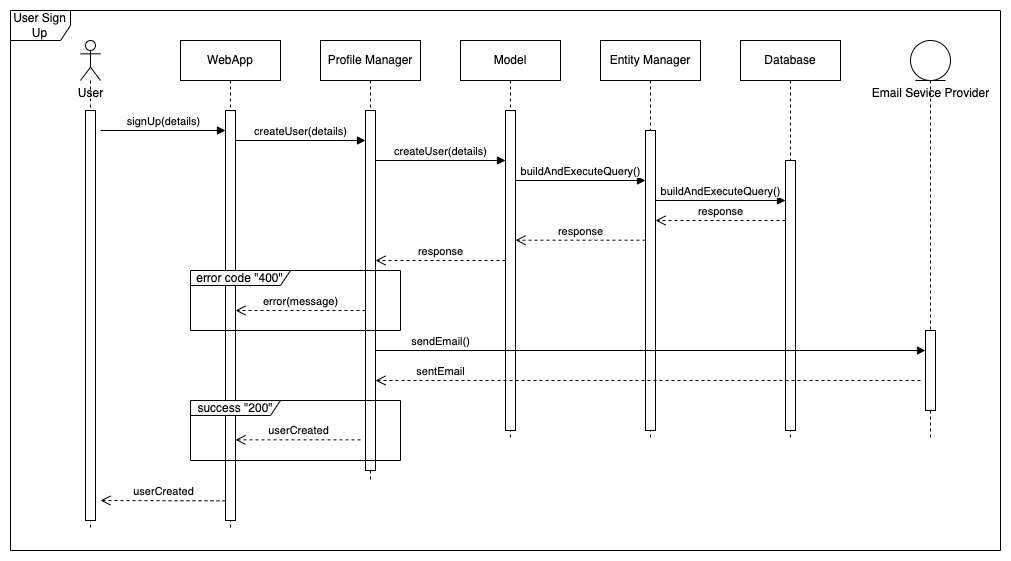
\includegraphics[width=0.8\textwidth]{Images/Sign_Up_Sequence_Diagram.png}
    \caption{\label{fig:metamodel9}[UC1] Sign Up Sequence Diagram.}
    \end{figure}
    \clearpage
    \item \textbf{User Log In} \\ \\
    The following diagram is the runtime sequence diagram for the User Log In use case. When a registered user tries a go on the S\&C WebApp and tries to log in an API request is sent from the client to the Profile Manager component in the web server along with the user entered credentials. These credentials are matched with the stored information in the database. If matched a token is generated by the Authenticate Manager and sent back to the client and the user's profile is visible.
    \begin{figure}[H]
    \centering
    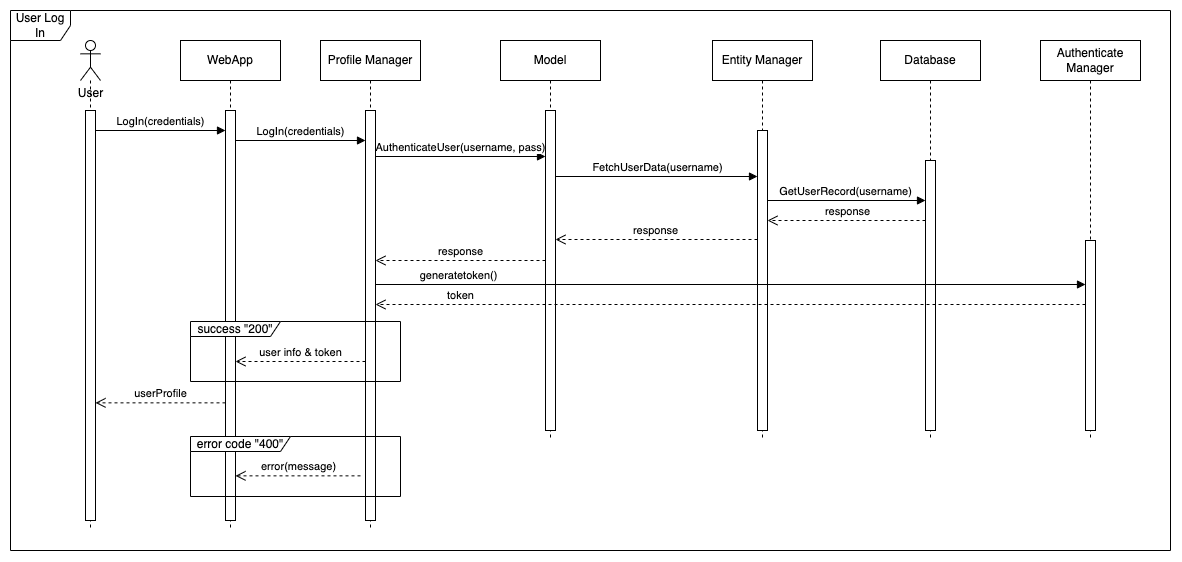
\includegraphics[width=0.8\textwidth]{Images/Log_In_Sequence_Diagram.png}
    \caption{\label{fig:metamodel9}[UC2] Log In Sequence Diagram.}
    \end{figure}
    \item \textbf{Creating CV} \\ \\
    The following diagram is the runtime sequence diagram for the Creating CV use case. A student user can create CV in the S\&C application which is used for applying for internship. For creation of CV the student fills out all the form present in the S\&C browser giving all details like education, skills, experiences etc. Once the user is satisfied the user can click on submit which calls the CreateCV API. The student's CV is ultimately saved in the database.
    \begin{figure}[H]
    \centering
    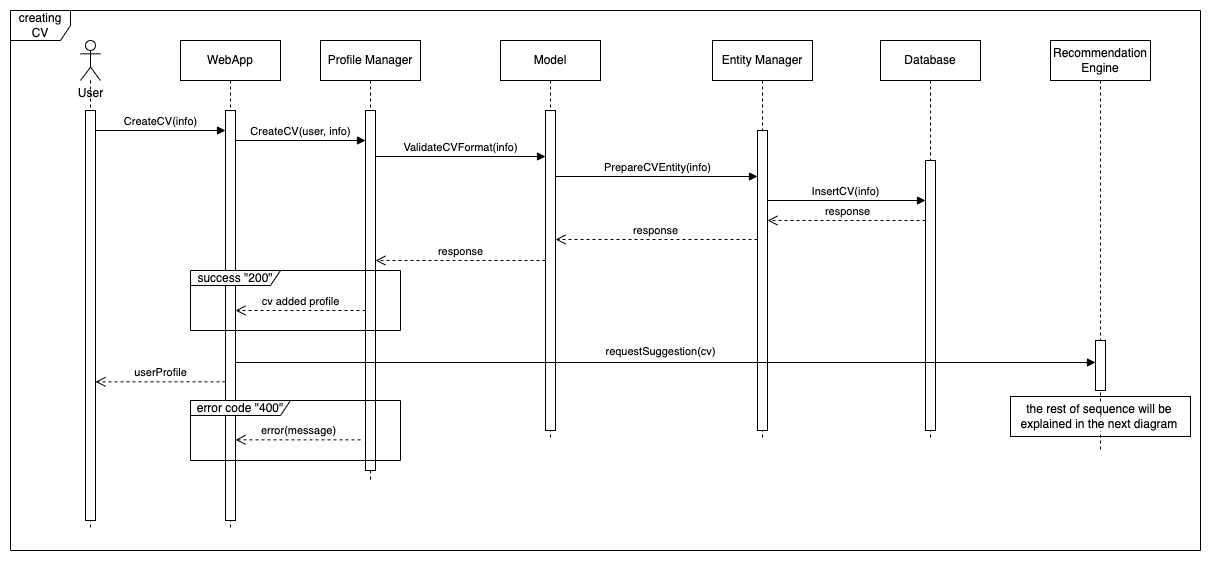
\includegraphics[width=0.8\textwidth]{Images/Creating_CV_Sequence_Diagram.png}
    \caption{\label{fig:metamodel9}[UC3] Creating CV Sequence Diagram.}
    \end{figure}
    \clearpage
    \item \textbf{Get Suggestions on CV} \\ \\
    While writing the CV, student can send requests to the Recommendation Engine in the application to get smart suggestions on the CV content. The Recommendation Engine analyzes the CV and provides tailored suggestions. These suggestions are displayed to the user, who can edit their CV based on the recommendations. Once the user finalizes and saves the edited CV, it is updated and stored in the system's database. The updated CV is reflected on the client-side. The following diagram illustrates the runtime sequence diagram for the Get Suggestions on CV use case.
    \begin{figure}[H]
    \centering
    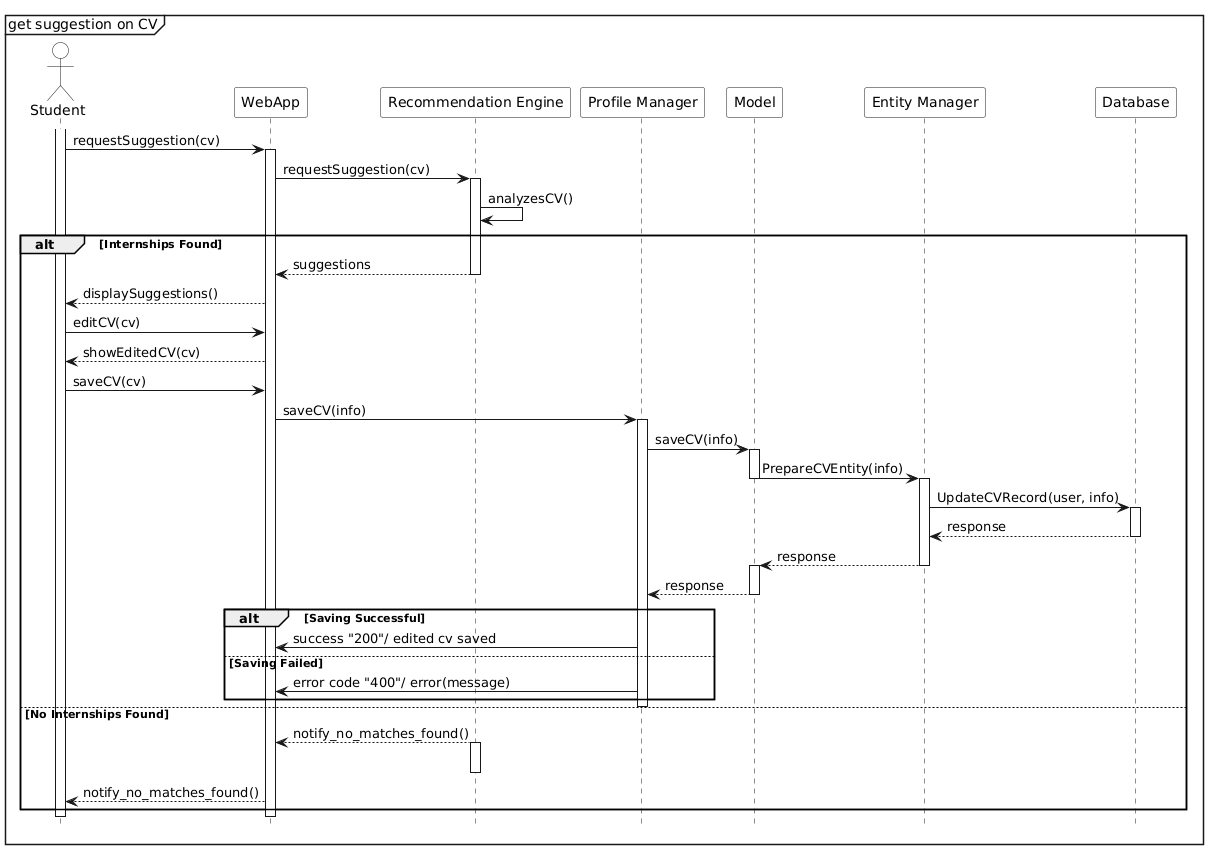
\includegraphics[width=0.8\textwidth]{Images/CV_Suggestion_Sequence_Diagram.png}
    \caption{\label{fig:metamodel9}[UC4] Get suggestion on CV Sequence Diagram.}
    \end{figure}
    \clearpage
    \item \textbf{Post Internship Advertisement} \\ \\
    After logging-in in the S\&C website a company recruiter can post internship advertisement. To post the user fills out all the necessary details related to the internship position like job description, skills required, compensation in the website and then clicks on "Post" button and all the details related to the job is then saved in the Database. The user is then returned to their profile where they can see the posted internship. The following diagram is the runtime sequence diagram for the Post Internship Advertisement use case.
    \begin{figure}[H]
    \centering
    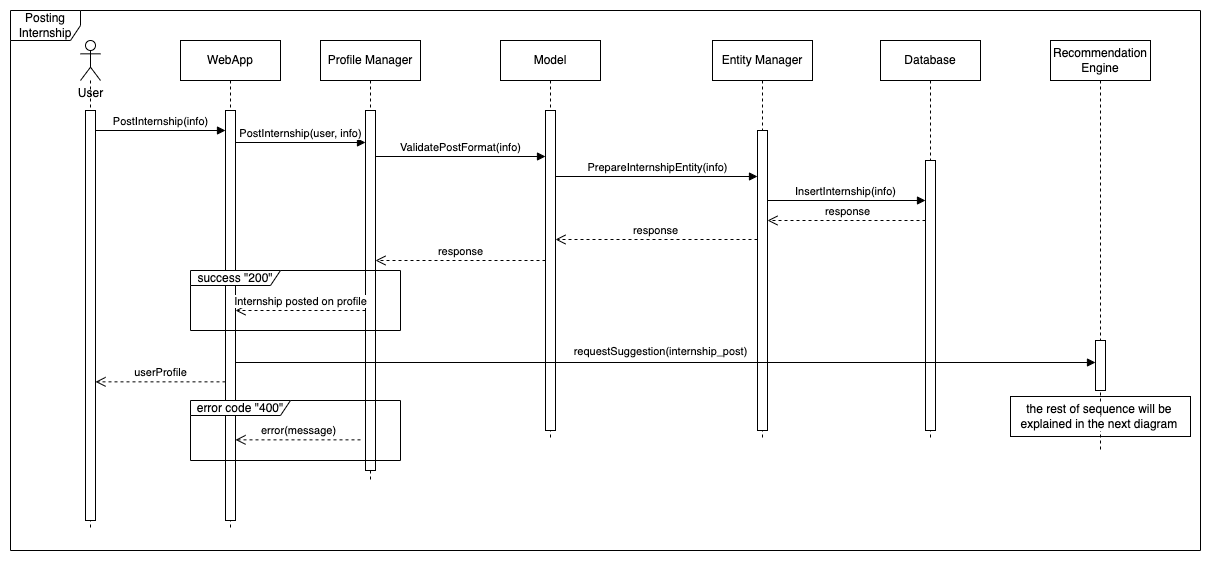
\includegraphics[width=0.8\textwidth]{Images/Posting_Internship_Sequence_Diagram.png}
    \caption{\label{fig:metamodel9}[UC5] Post Internship Sequence Diagram.}
    \end{figure}
    \clearpage
    \item \textbf{Get Suggestions on Ad} \\ \\
    During the writing of an internship advertisement, companies can request suggestions from the S\&C system to enhance the post. The content of the job post is sent to the Recommendation Engine, which analyzes the content and provides suggestions to improve the advertisement. These suggestions are displayed to the company user, who can either edit and finalize the ad or reject the suggestions. Once the edited advertisement is saved, it is updated in the system and reflected in the database. The following diagram illustrates the runtime sequence diagram for the Get Suggestions on Ad use case.
    \begin{figure}[H]
    \centering
    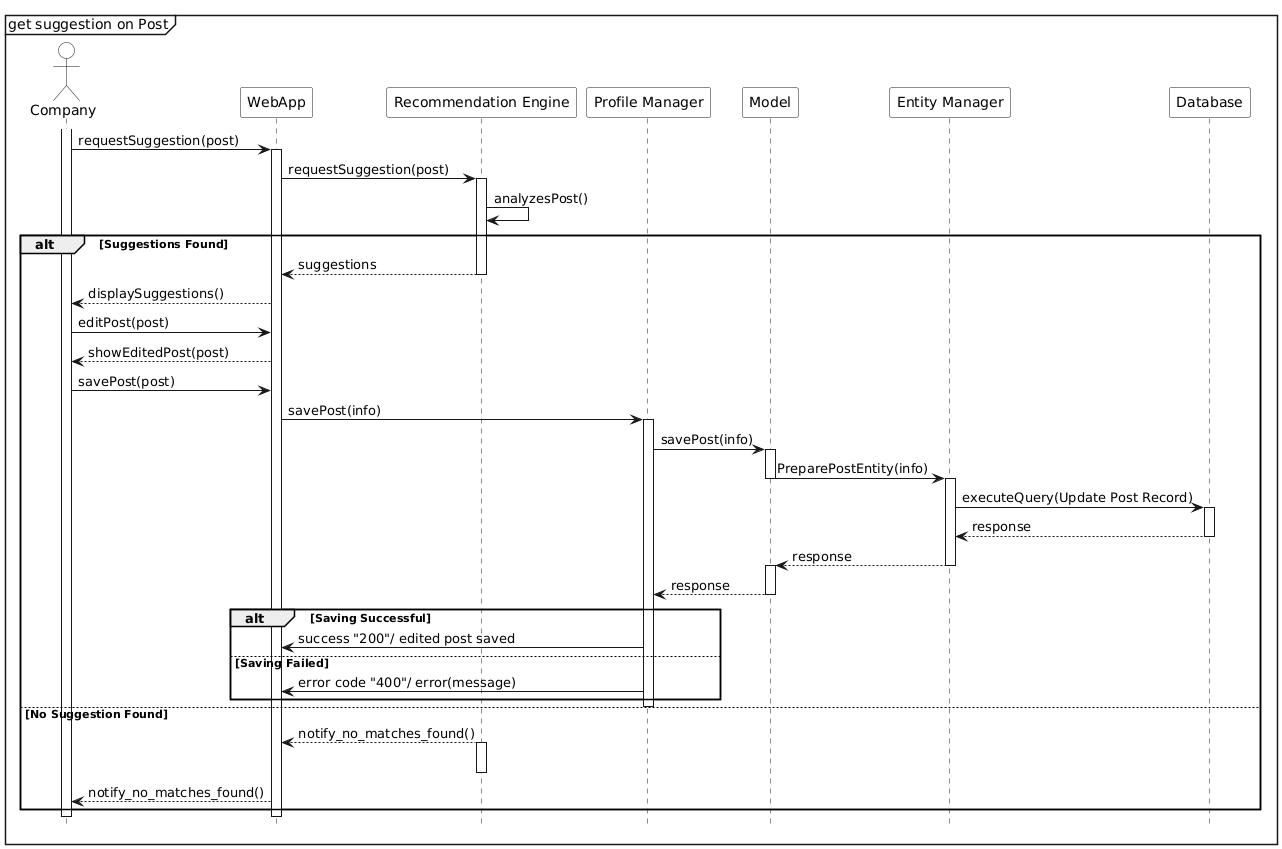
\includegraphics[width=0.8\textwidth]{Images/Internship_Suggestion_Sequence_Diagram.png}
    \caption{\label{fig:metamodel9}[UC6] Get suggestion on Internship Post Advertisement Sequence Diagram.}
    \end{figure}
    \item \textbf{Define a Questionnaire} \\ \\
    After posting an internship post the company personnel can create a Questionnaire to be sent to the students who are shortlisted for the next step. The company personnel can define the questionnaire for a particular internship offer by fetching details of the internship from the server. Once satisfied the user saves then questionnaire in the database for later use. The following diagram is the runtime sequence diagram for the Define a Questionnaire use case.
    \begin{figure}[H]
    \centering
    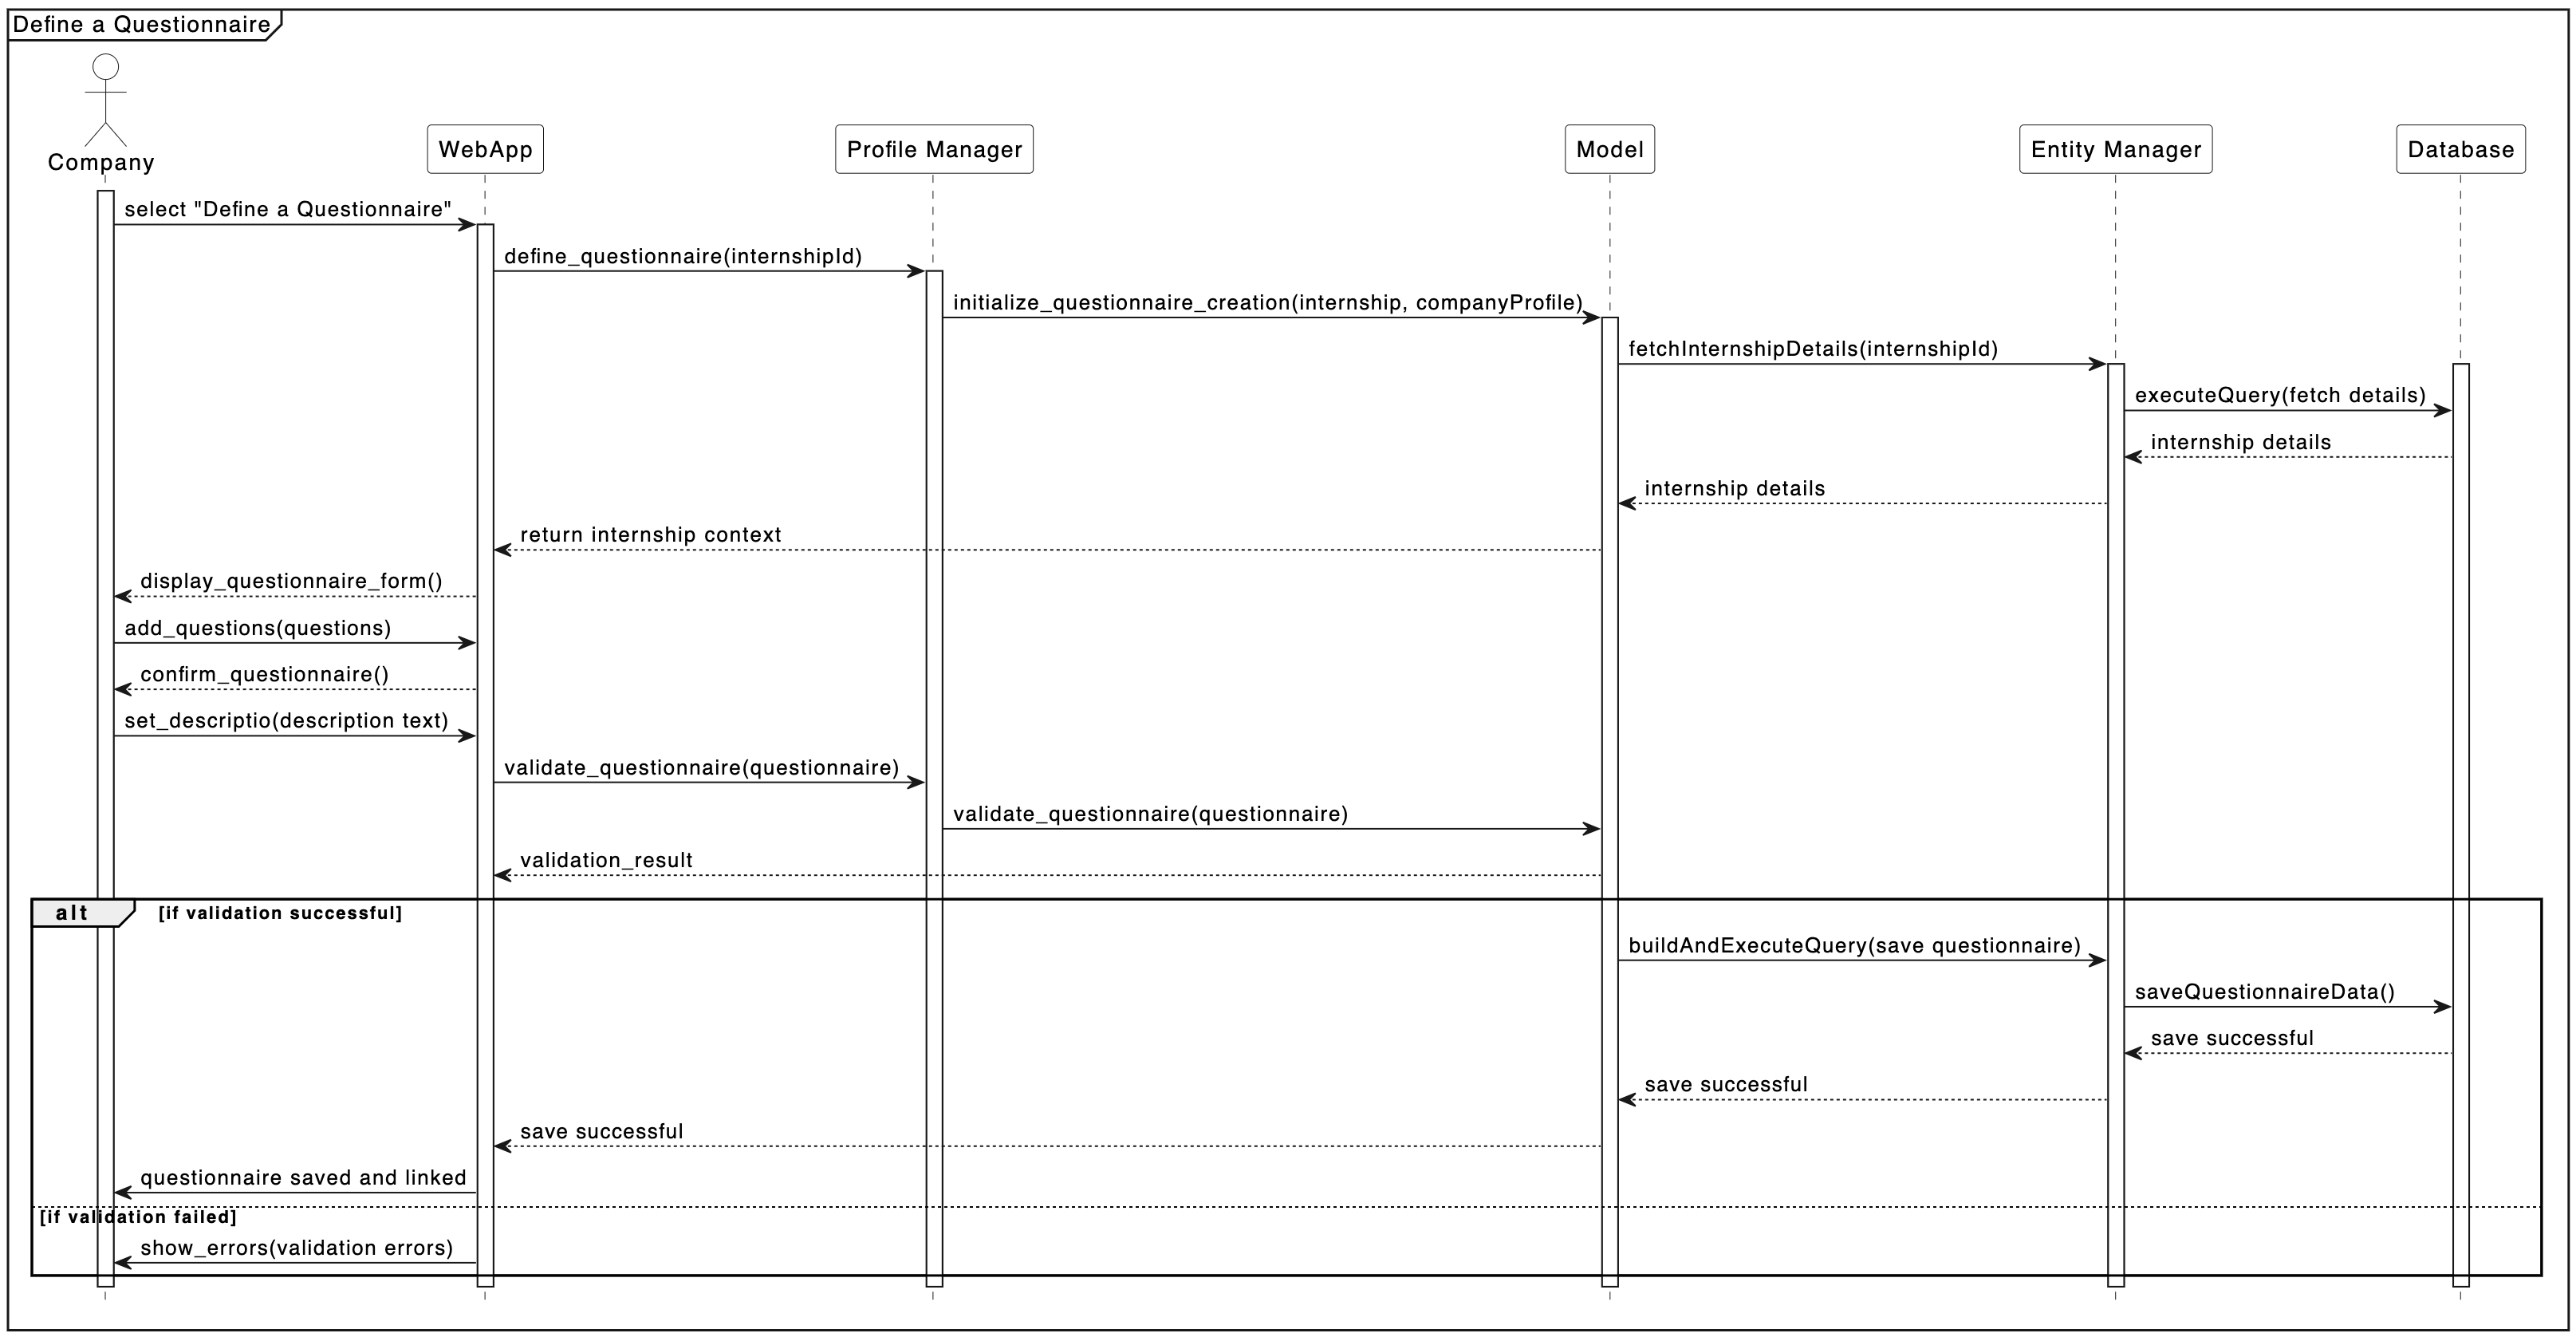
\includegraphics[width=0.8\textwidth]{Images/Define_Questionnaire_Sequnce_Diagram.png}
    \caption{\label{fig:metamodel9}[UC7] Define a Questionnaire for the Internship Post Sequence Diagram.}
    \end{figure}
    \item \textbf{Search Internship} \\ \\
    Students can search for internship by typing required keywords like job roles, position, location in the search internship tab of the S\&C website. ElasticSearch will be used for filtering and available internships are sent to the student. The student can then open each internship and view it's details. The following diagram is the runtime sequence diagram for the Search Internship use case.
    \begin{figure}[H]
    \centering
    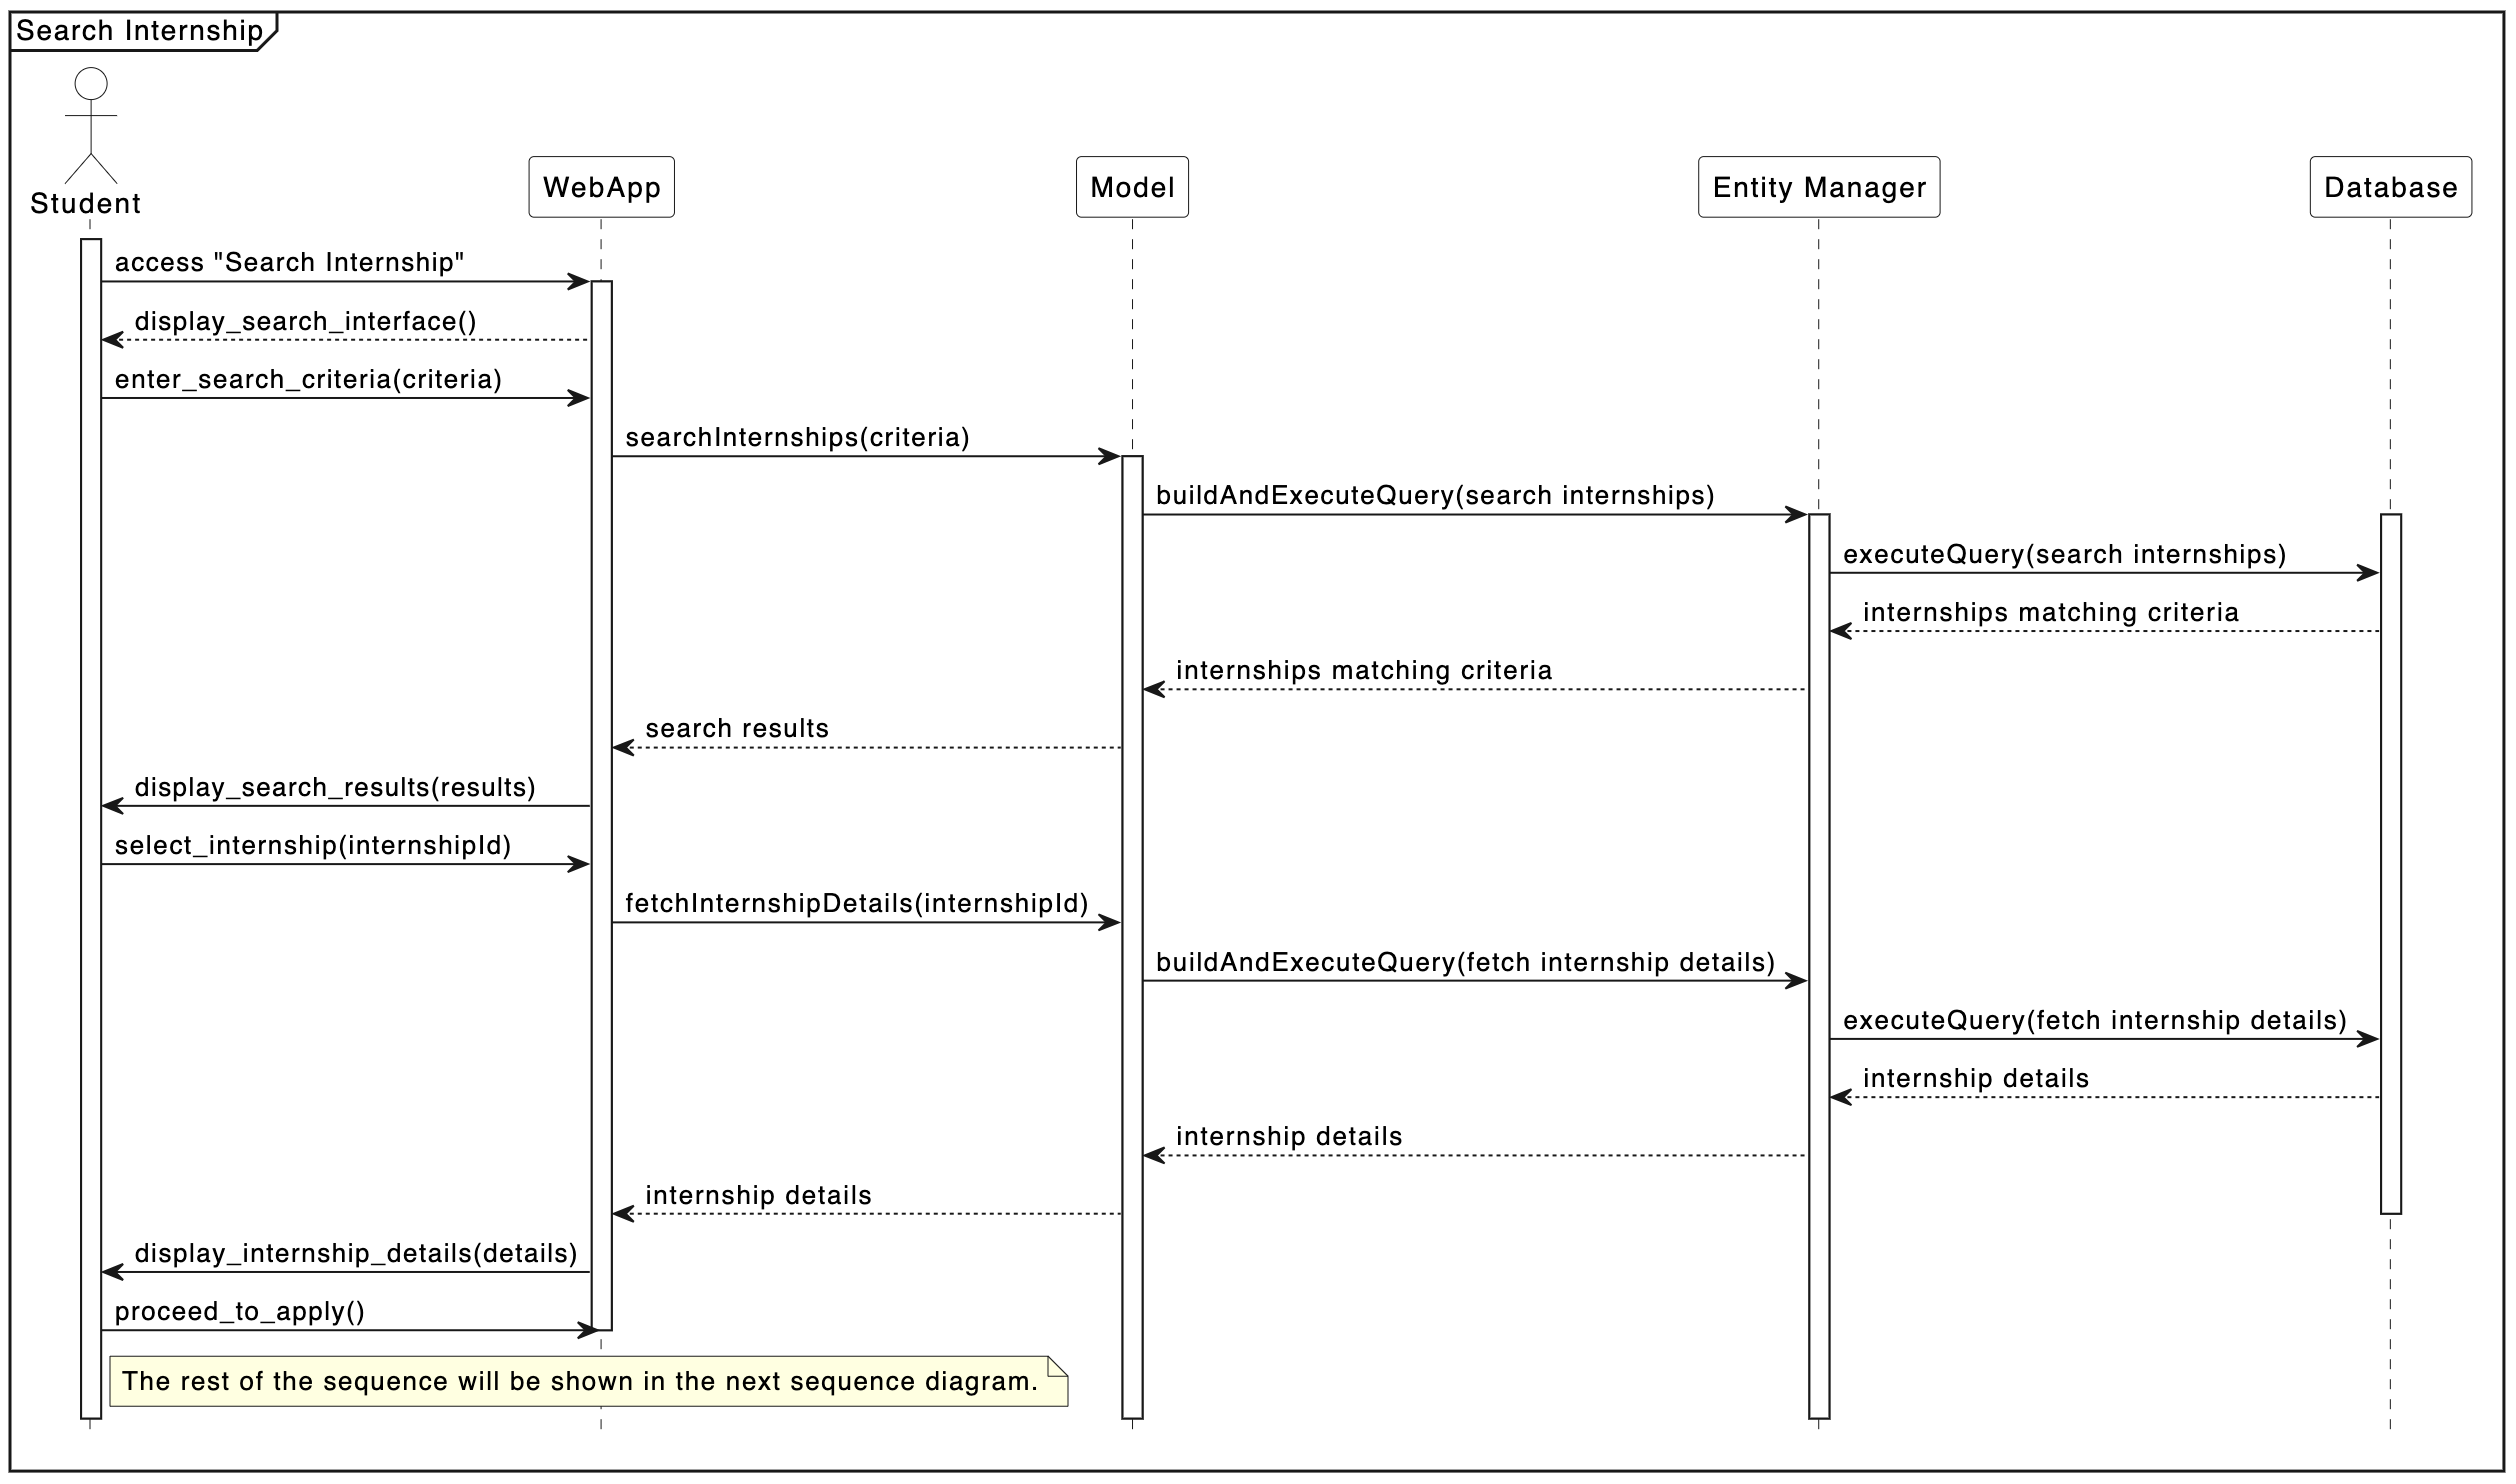
\includegraphics[width=0.8\textwidth]{Images/Search_Internship_Sequence_Diagram.png}
    \caption{\label{fig:metamodel9}[UC8] Search Internship Sequence Diagram.}
    \end{figure}
    \item \textbf{Apply Internship} \\ \\
    A student can apply to any desired internship post by clicking on the "Apply" button. Student will be prompted to select application materials like CV, cover letter. Once selected the students application for that internship will be saved in the database. Once applied is submitted Notification Manager will send notification to the company. The following diagram is the runtime sequence diagram for the Apply Internship use case.
    \begin{figure}[H]
    \centering
    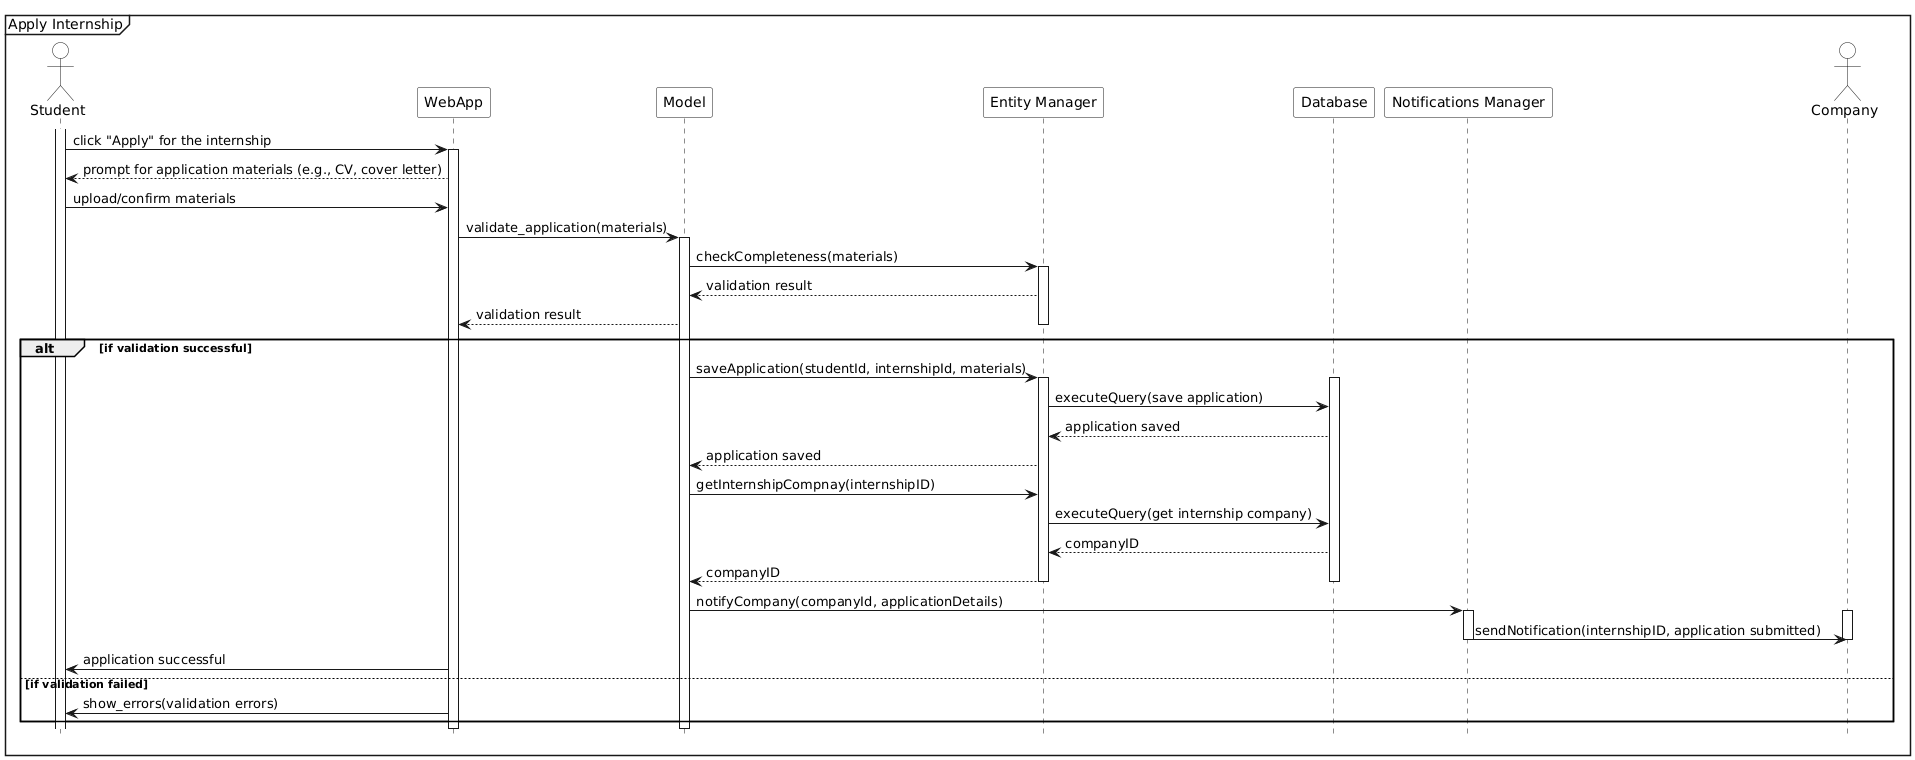
\includegraphics[width=0.8\textwidth]{Images/Apply_Internship_Sequence_Diagram.png}
    \caption{\label{fig:metamodel9}[UC9] Apply Internship Sequence Diagram.}
    \end{figure}
    \item \textbf{Accept/Reject Application} \\ \\
    A company recruiter can view the applications of students who have applied for their internship post. Company recruiter can fetch the the list of all applicants. Then user then clicks on "Accept" or "Reject" for all applications for the next step. The students are notified of the same. The application status of each application is then updated accordingly in the database. The following diagram is the runtime sequence diagram for the Accept/Reject Application use case.
    \begin{figure}[H]
    \centering
    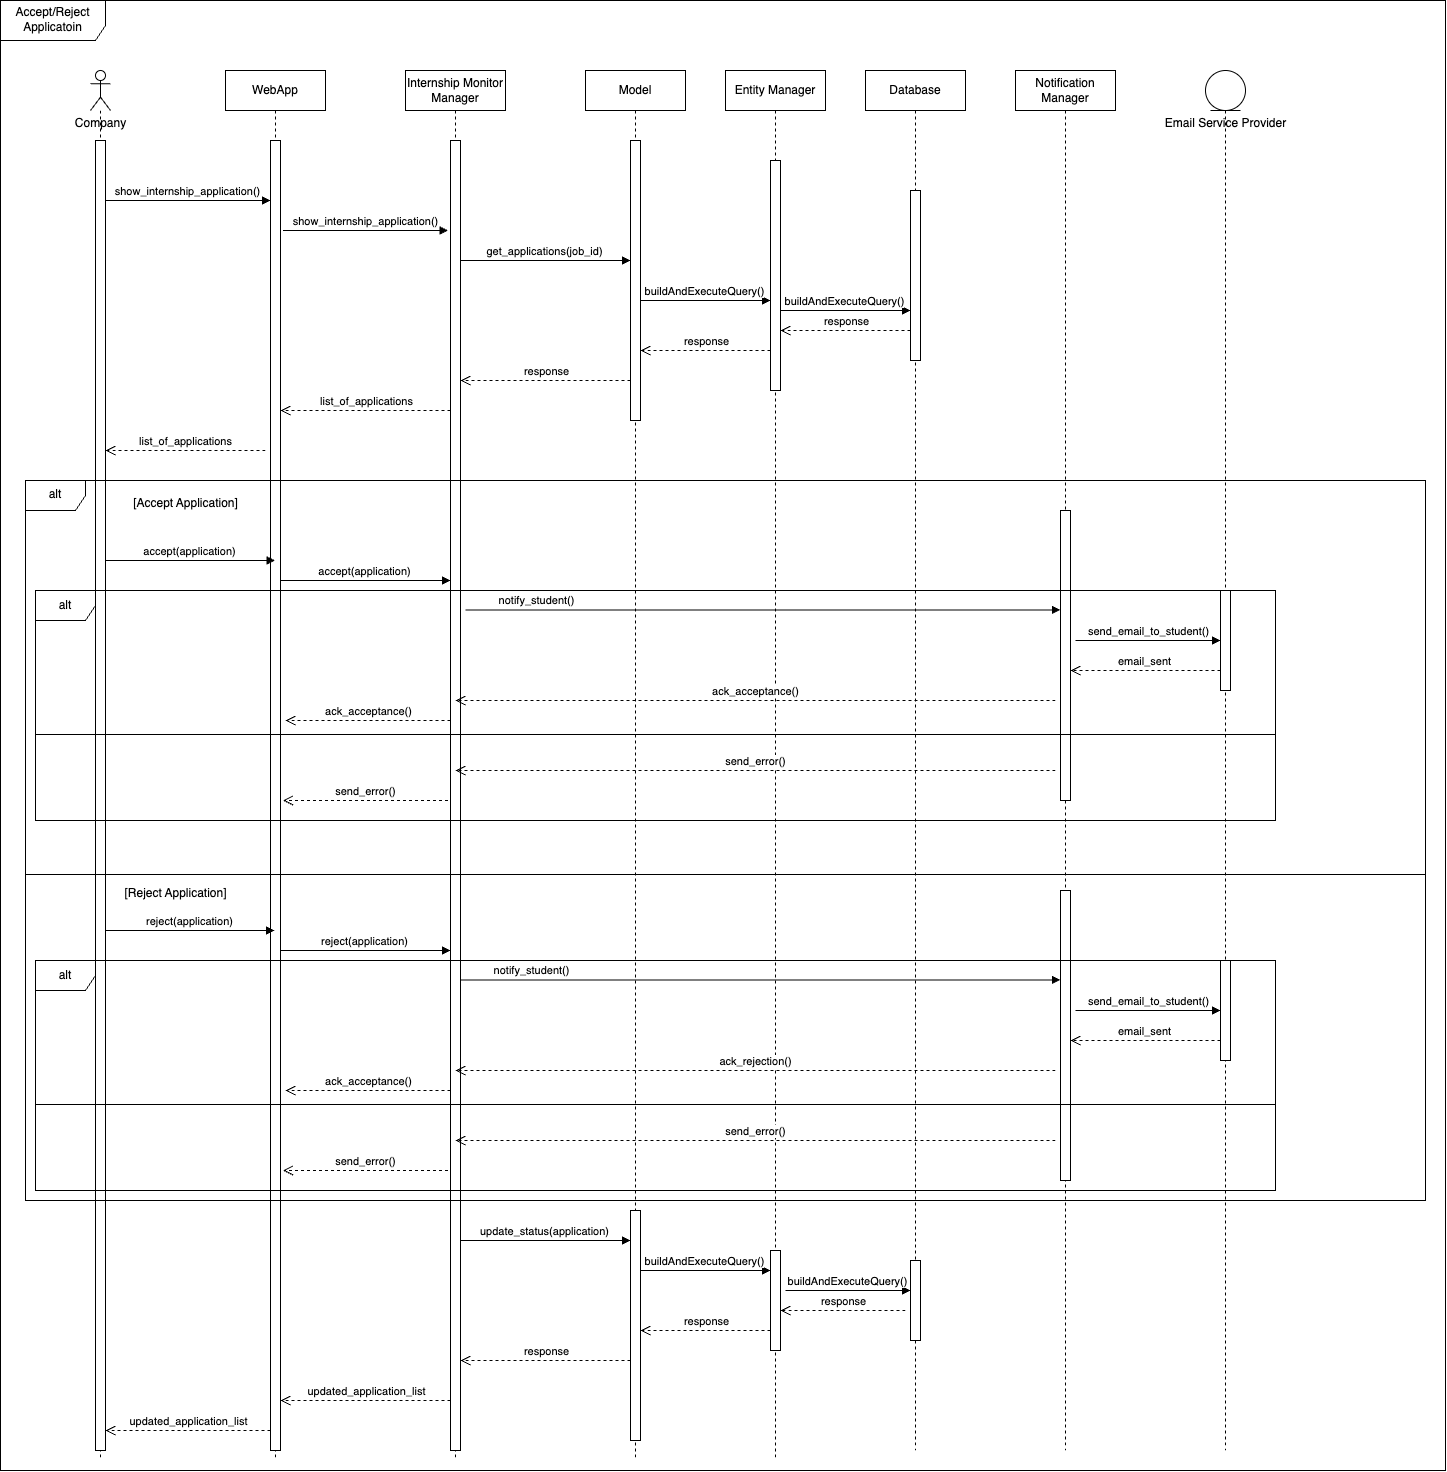
\includegraphics[width=0.8\textwidth]{Images/Accept_reject_sequence_diagram.png}
    \caption{\label{fig:metamodel9}[UC10] Accept/Reject Application Sequence Diagram}
    \end{figure}
    \item \textbf{Match Students and Internships} \\ \\
    In S\&C platform matchmaking system is there to notify students of available internship and notify companies and eligible students with required characteristics for an open internship are available. Recommendation Engine analyses CVs of students and descriptions of internships and for each student creates list of suitable companies and for each company creates list of suitable candidates and notifies each parties using email. This recommendation process is carried out at a periodic interval (for e.g. every 24 hours). The following diagram is the runtime sequence diagram for the Match Student and Internship Sequence Diagram use case.
    \begin{figure}[H]
    \centering
    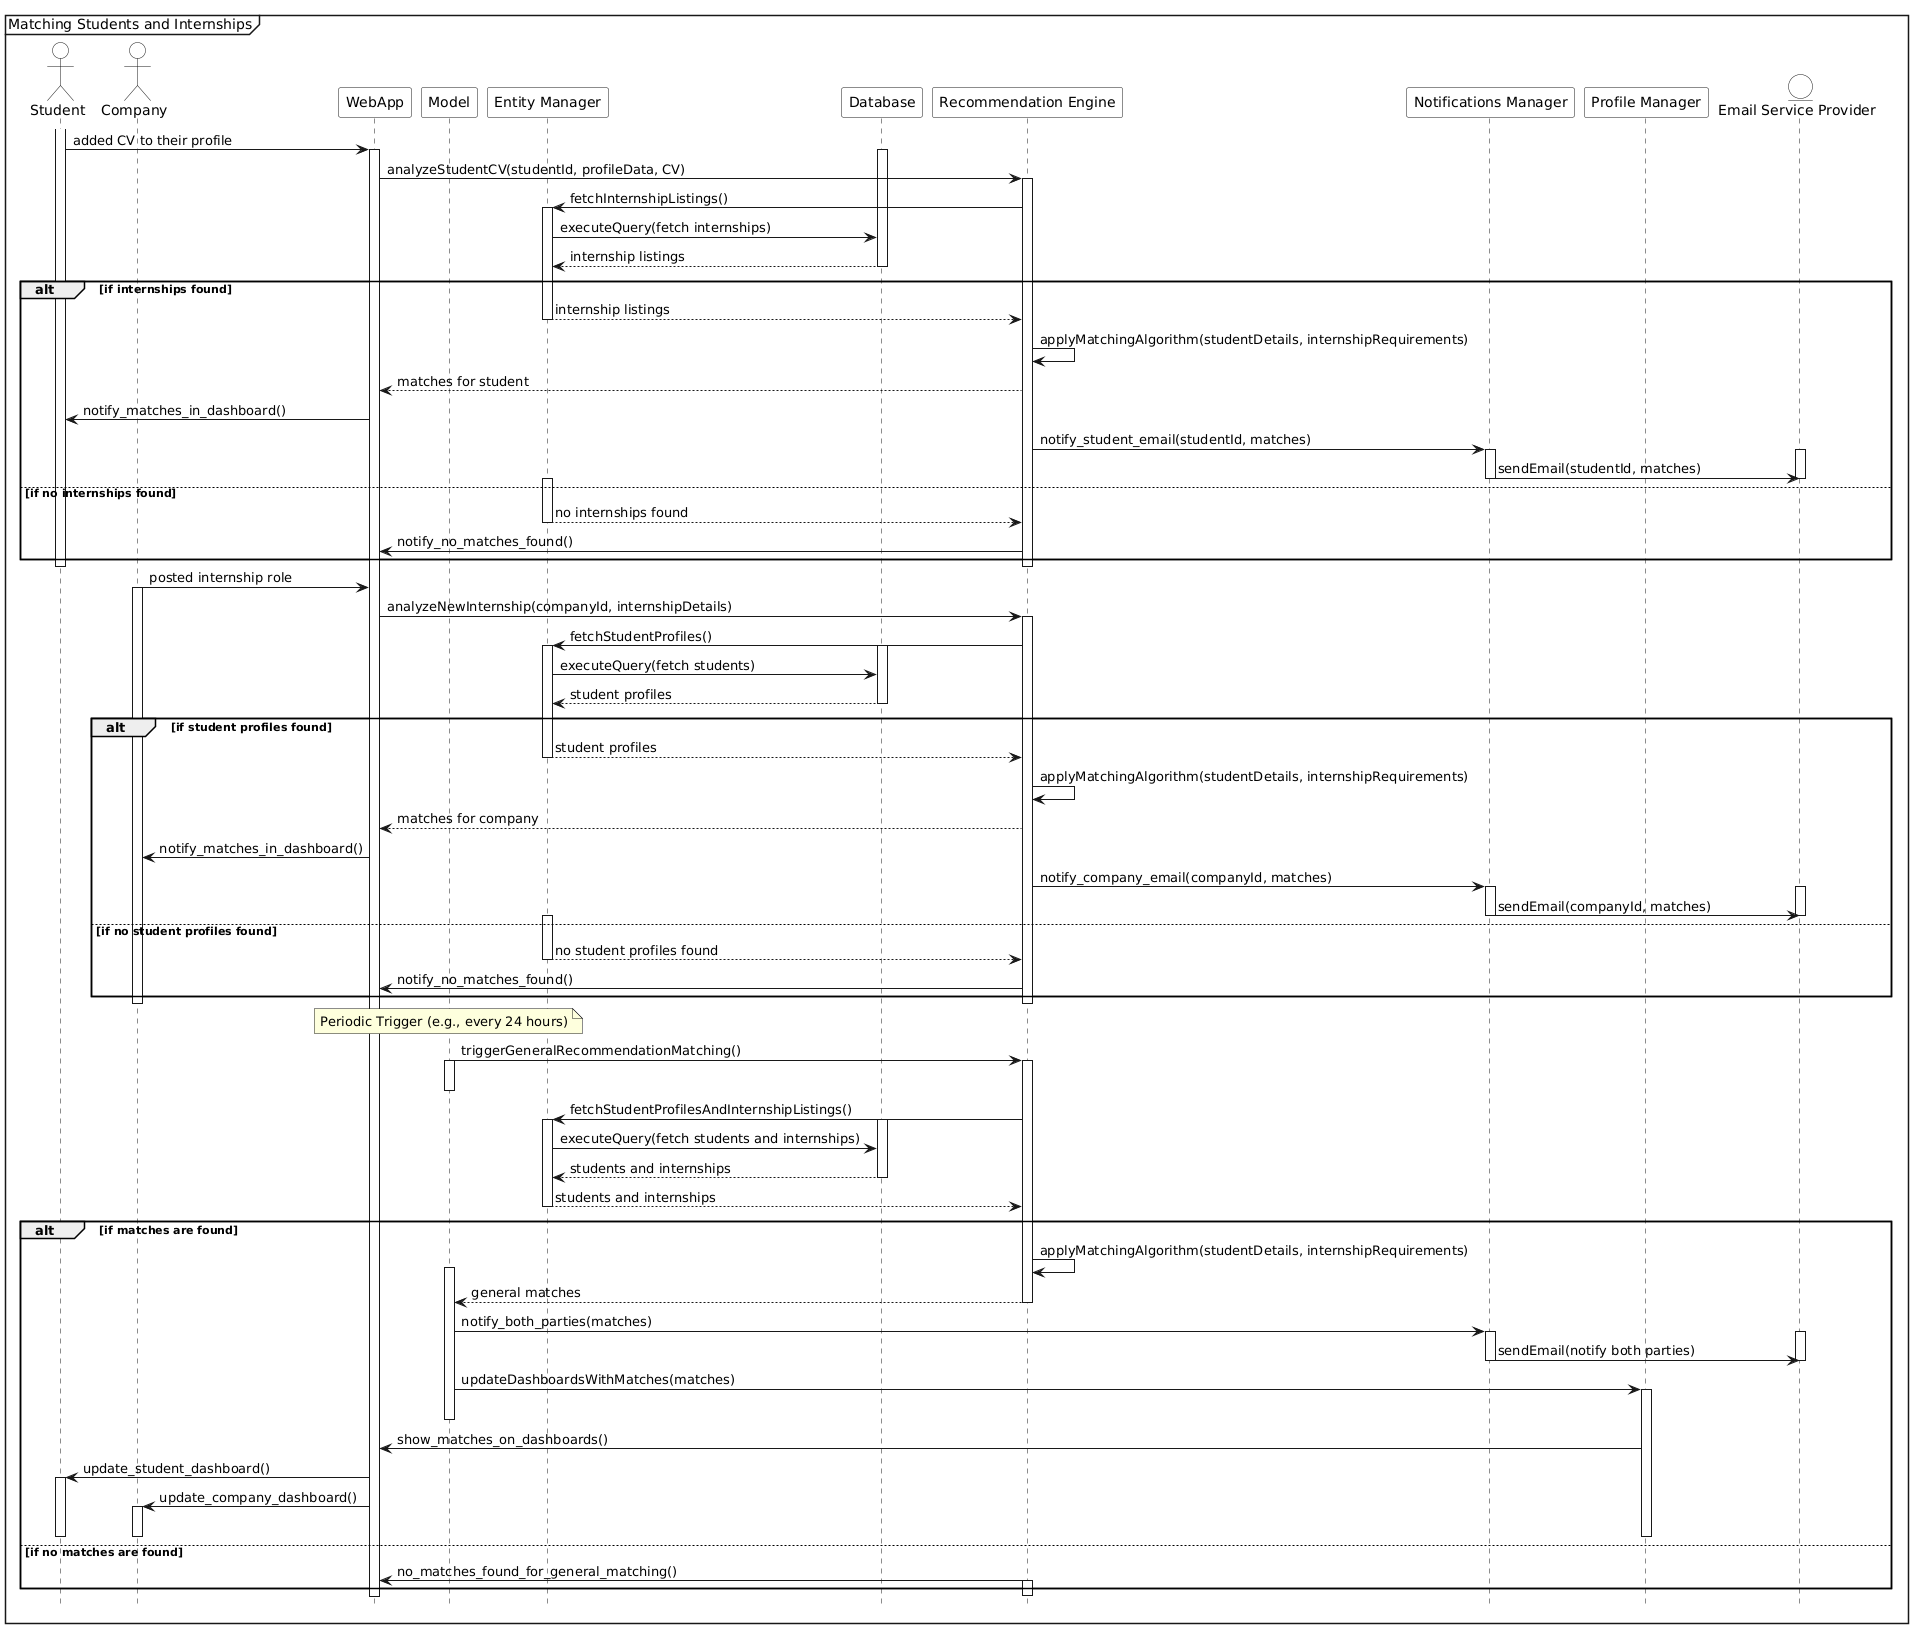
\includegraphics[width=0.8\textwidth]{Images/Match_Student_Internship_Sequence_diagram.png}
    \caption{\label{fig:metamodel9}[UC11] Match Student and Internship Sequence Diagram}
    
    \end{figure}
    \item \textbf{Selection Process} \\ \\
    Once a company accepts an application or a match-making recommendation is accepted by both the company and student the selection process starts. A communication channel is opened between the company and the student both the parties are notified. The previously defined questionnaire is forwarded to the student to be answered. The Student then fills up the questionnaire and submits it which is then can be read by the company. The company can then either select the student for the interview or reject them. In the both the cases the students will be notified and the selected student will be added to the interview shortlist. The following diagram is the runtime sequence diagram for the Selection Process Sequence Diagram use case.
    \begin{figure}[H]
    \centering
    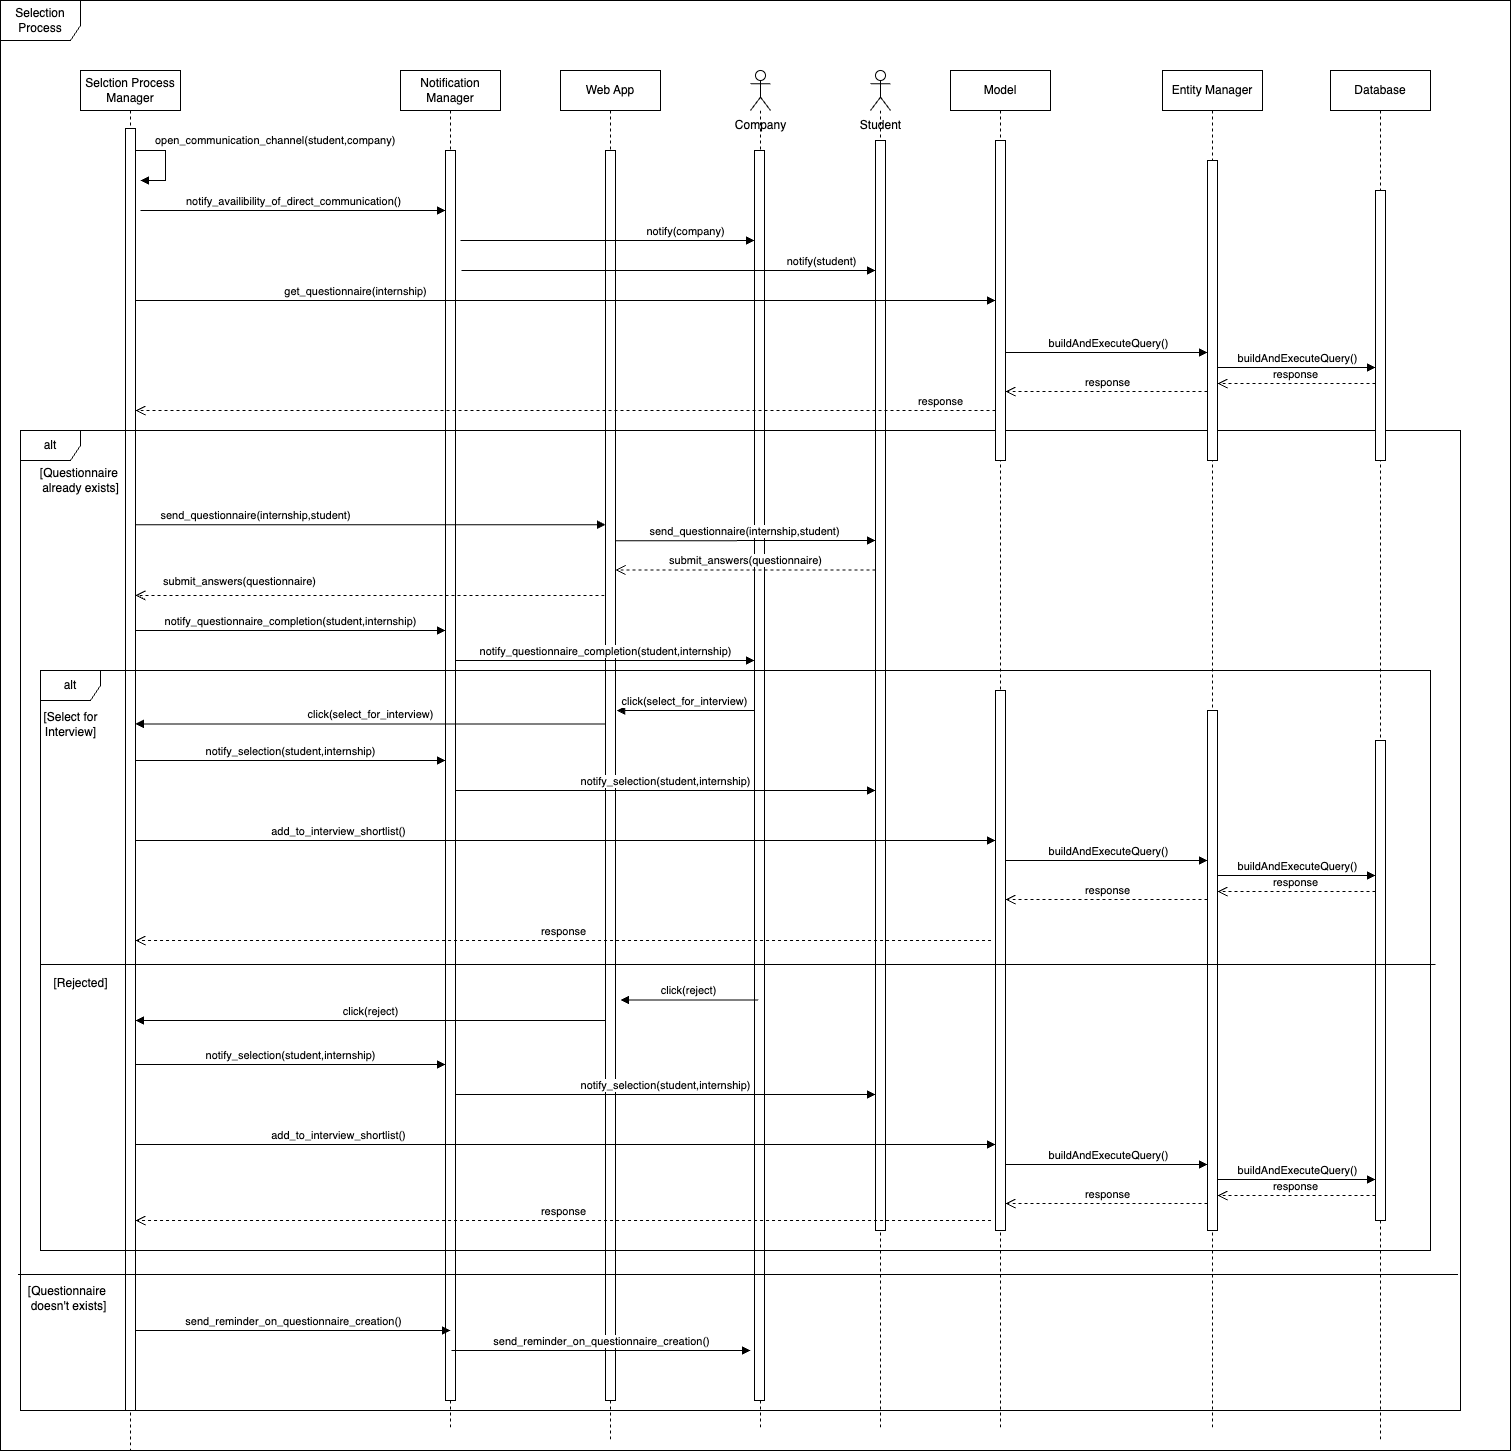
\includegraphics[width=0.8\textwidth]{Images/select_process_seq_diag.png}
    \caption{\label{fig:metamodel9}[UC12] Selection Process Sequence Diagram}
    \end{figure}
    
    \item \textbf{Set Up Interview (S\&C Platform Manage Interview Process)} \\ \\
    Once company selects a student for interview the Selection Process Manager will request both student and company to select range of available dates in the calender. Once dates are selected an interview date will be selected and interview details along with dates and location or interview link will be sent to both the student and company using Notification Manager and the data will be saved in the database. The following diagram is the runtime sequence diagram for the Set Up Interview (S\&C Platform Manage Interview Process) Sequence Diagram use case.
    \begin{figure}[H]
    \centering
    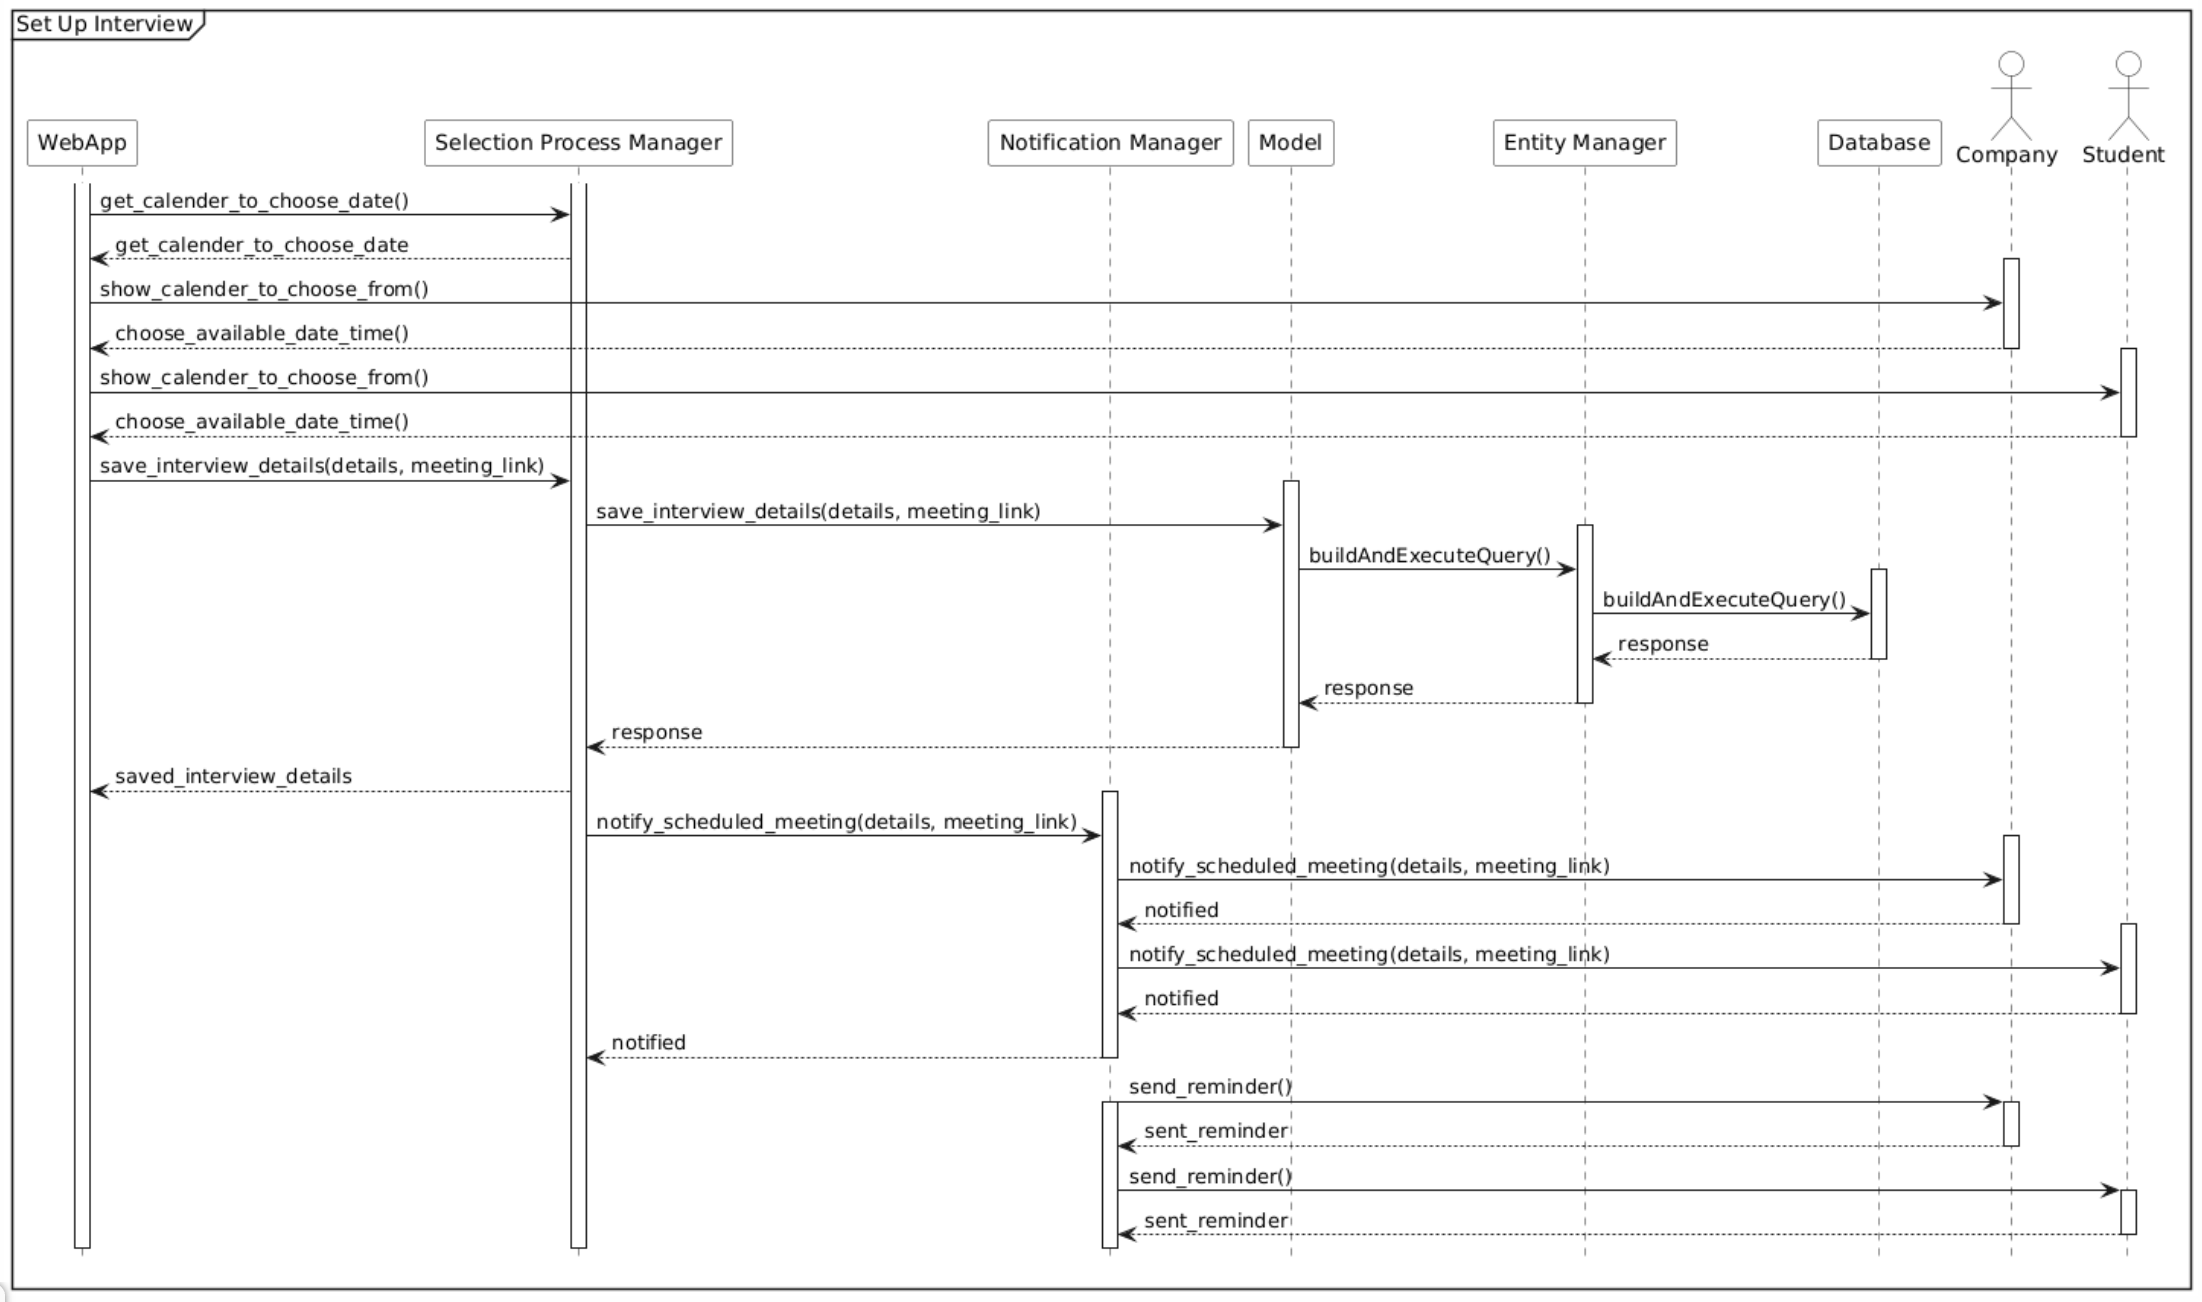
\includegraphics[width=0.8\textwidth]{Images/set_up_interview_sequence1.png}
    \caption{\label{fig:metamodel9}[UC13] Set Up Interview Sequence Diagram}
    \end{figure}
    \item \textbf{Finalize Decision (company finalize the decision for selection process)} \\ \\
    Company can see the lift of the interview students and from there hire or reject a student for that post. If the company decides to hire a student notification is sent to that student. If the company rejects then notification is sent to that student. The decisions are then updated in the databases. If no students have been interviewed yet it is reflected in the website. The following diagram is the runtime sequence diagram for the Finalize Decision Sequence Diagram use case.
    \begin{figure}[H]
    \centering
    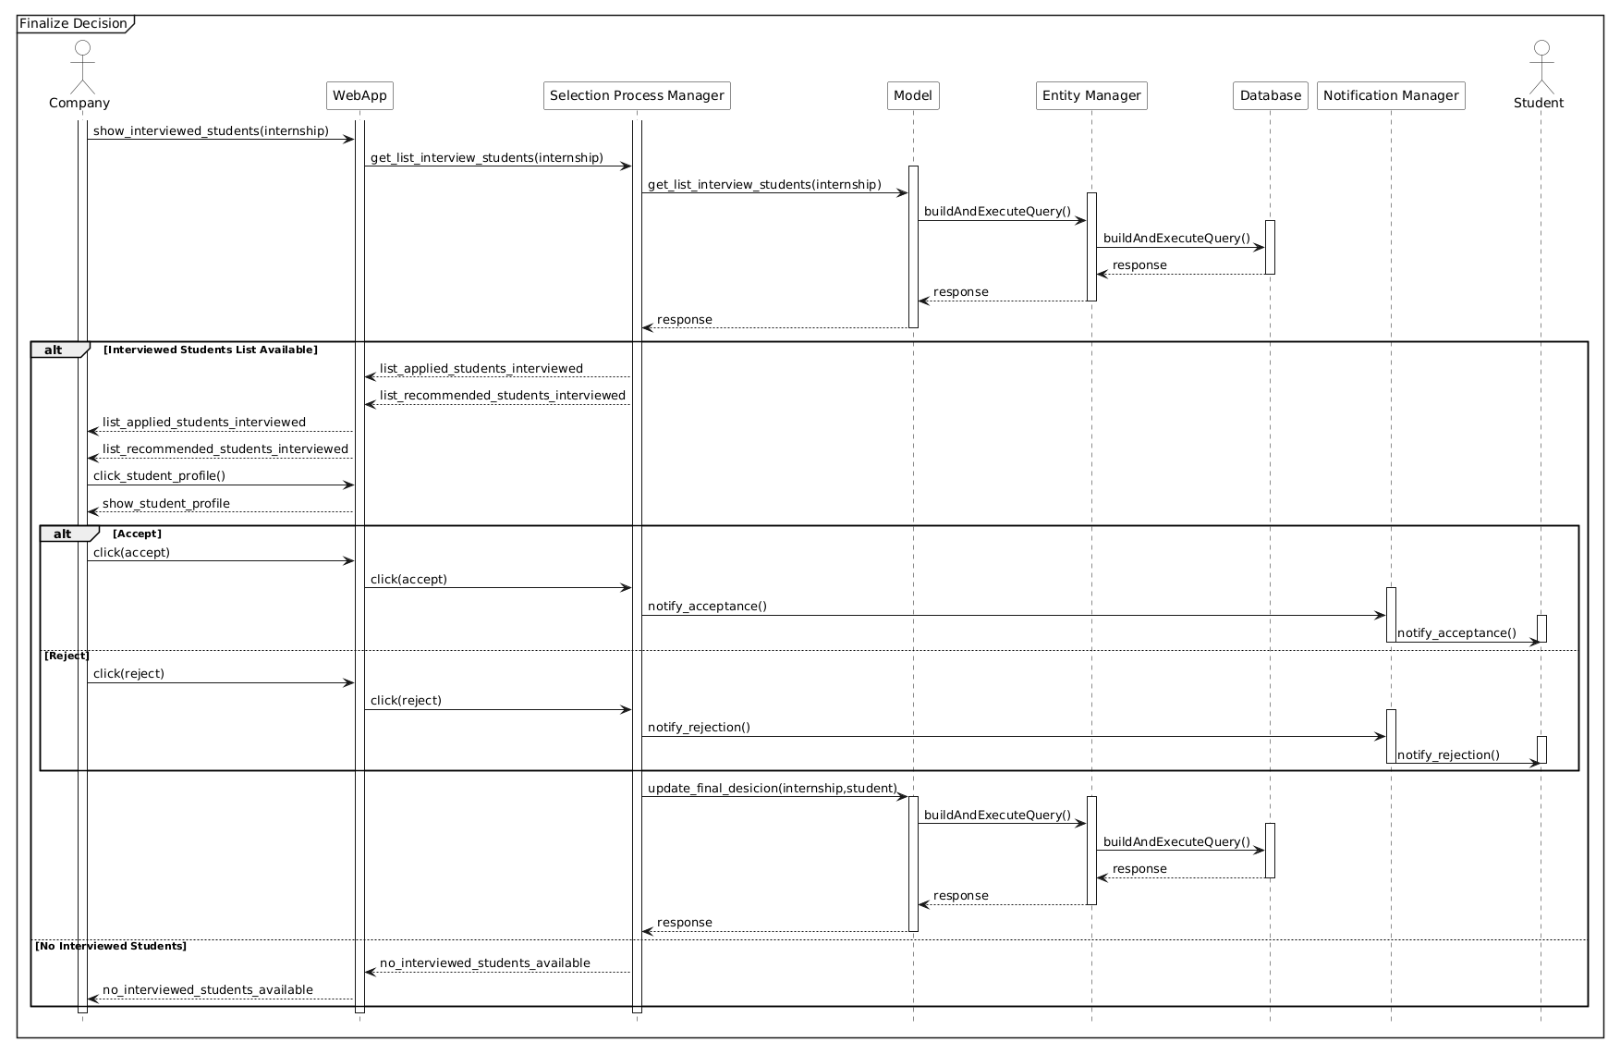
\includegraphics[width=0.8\textwidth]{Images/Finalize-decision-sequence-diagram.png}
    \caption{\label{fig:metamodel9}[UC14] Set Up Interview Sequence Diagram}
    \end{figure}
    \clearpage
    \item \textbf{Collect Feedback} \\ \\
    After completion of the interview or while using of the application the students and companies are requested by the Feedback and Analytics manager to give feedback on the website and it's applications. The feedback given by the users are send saved in the database. The feedback is then used by the developers of the system to improve the recommendation engine. After improvement the recommendation engine can suggest better and more accurate matches to students and companies. The following diagram is the runtime sequence diagram for the Collect Feedback Sequence Diagram use case.
    \begin{figure}[H]
    \centering
    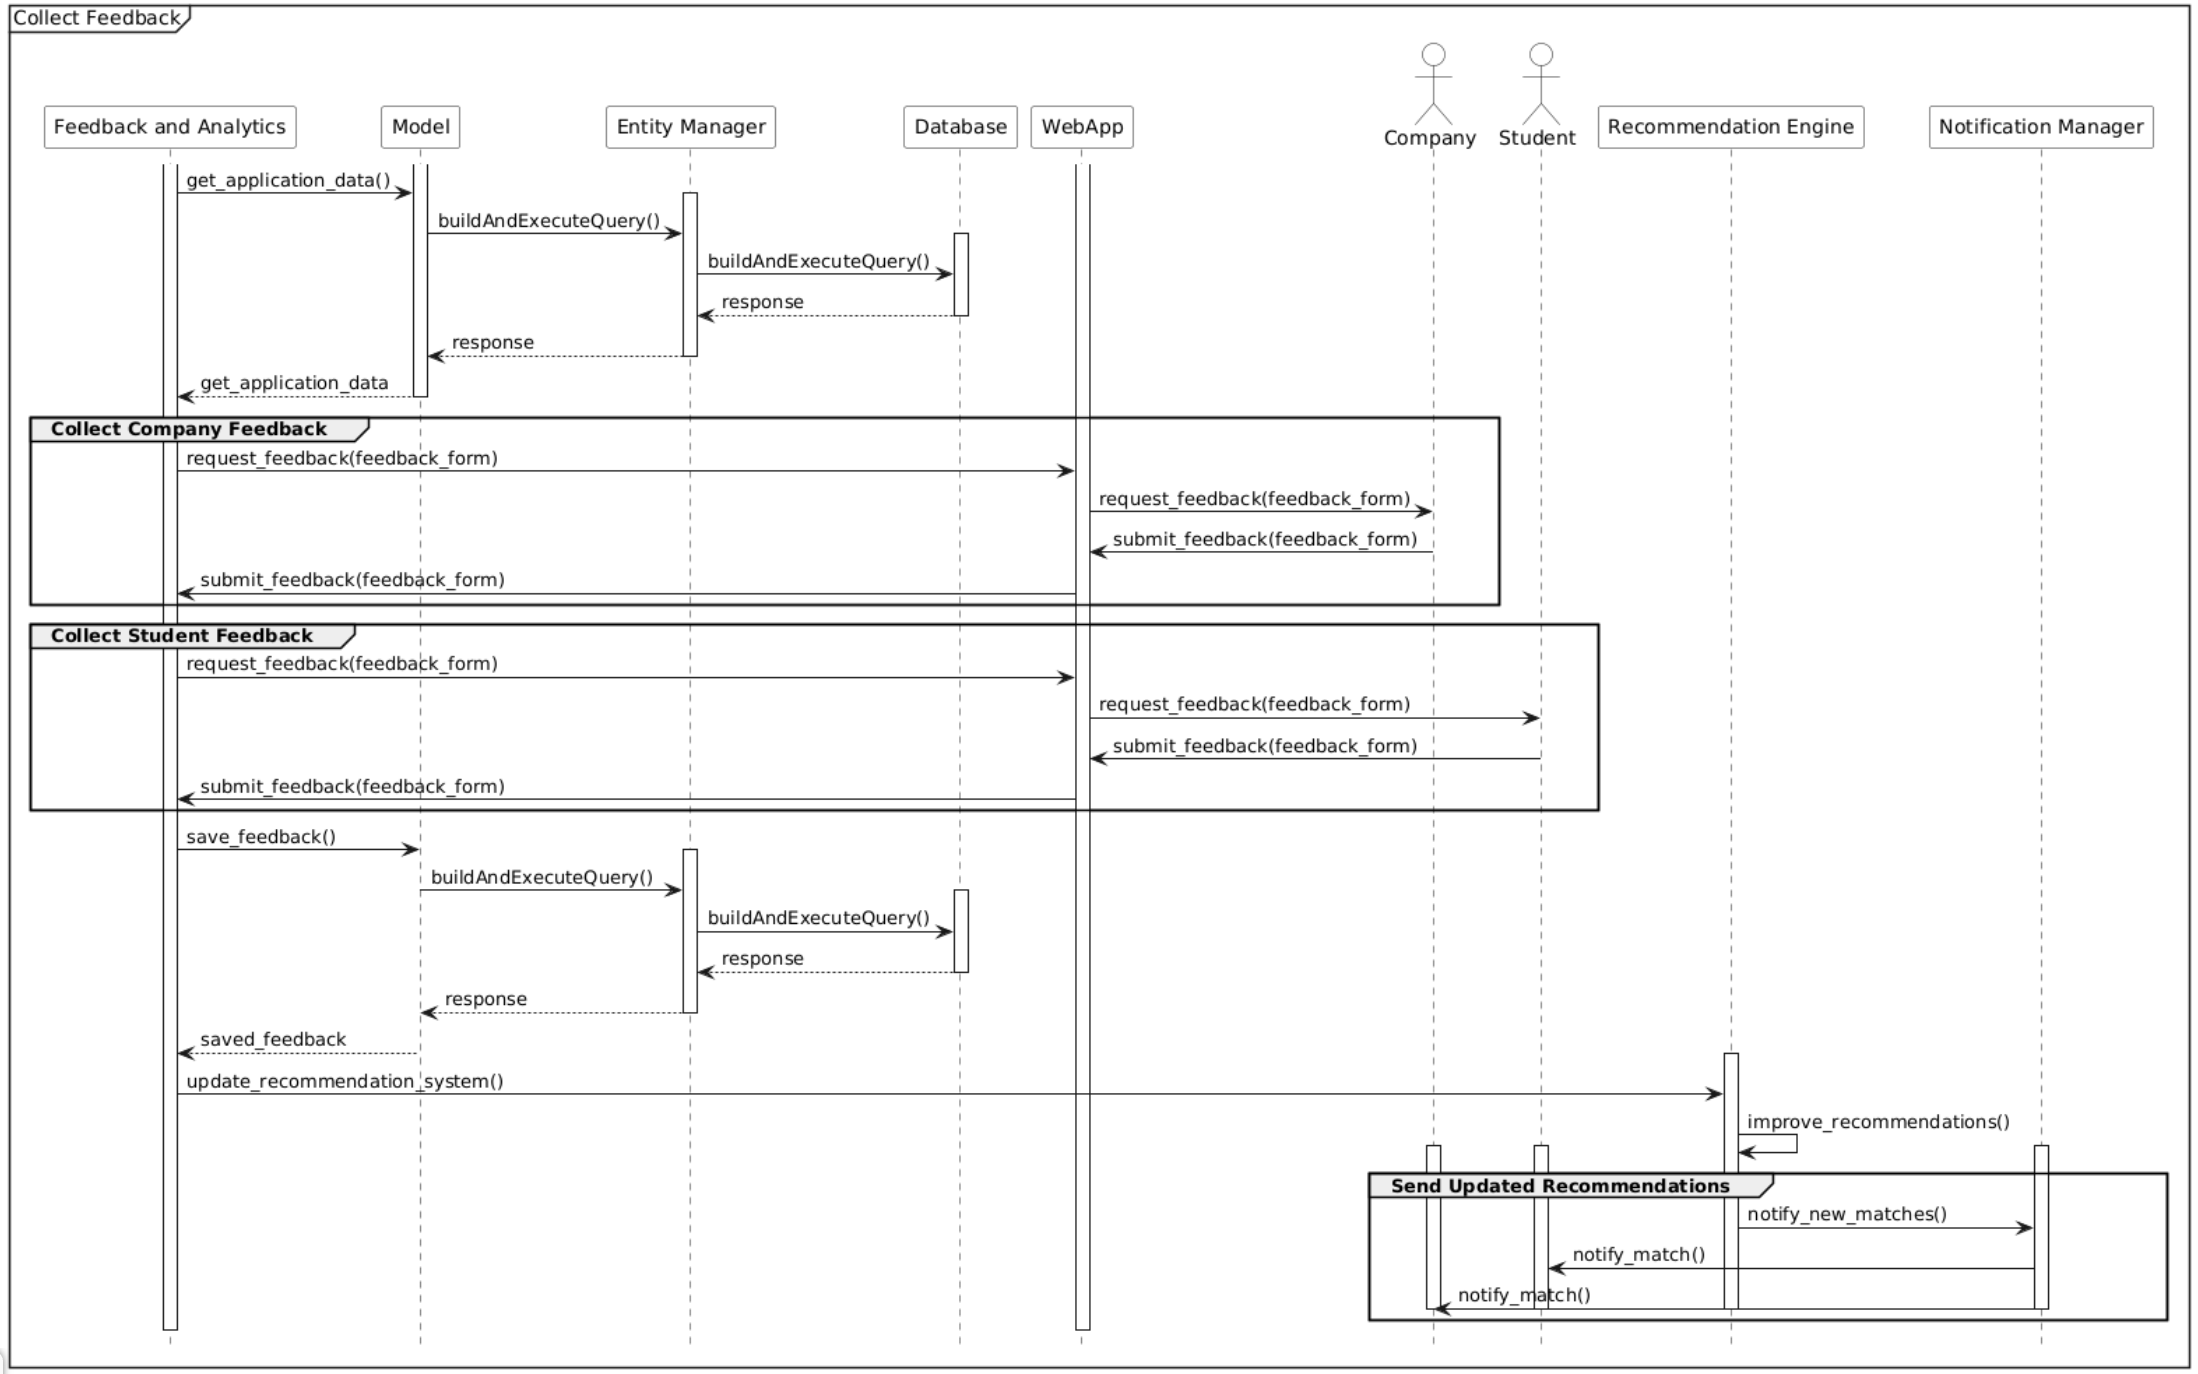
\includegraphics[width=0.8\textwidth]{Images/Collect Feedback sequence diagram.png}
    \caption{\label{fig:metamodel9}[UC15] Collect Feedback Sequence Diagram}
    \end{figure}
    \clearpage
    \item \textbf{Monitor Internship Status} \\ \\
    Users can monitor the internship status. University can monitor internships of it's students. After login university administrator can go to university's profile page and from there can see the list of their students. For each students university administrator can get the internship details and progress from database which is handled by Internship Monitor Manager. The following diagram is the runtime sequence diagram for the Internship Monitor Manage Sequence Diagram use case.
    \begin{figure}[H]
    \centering
    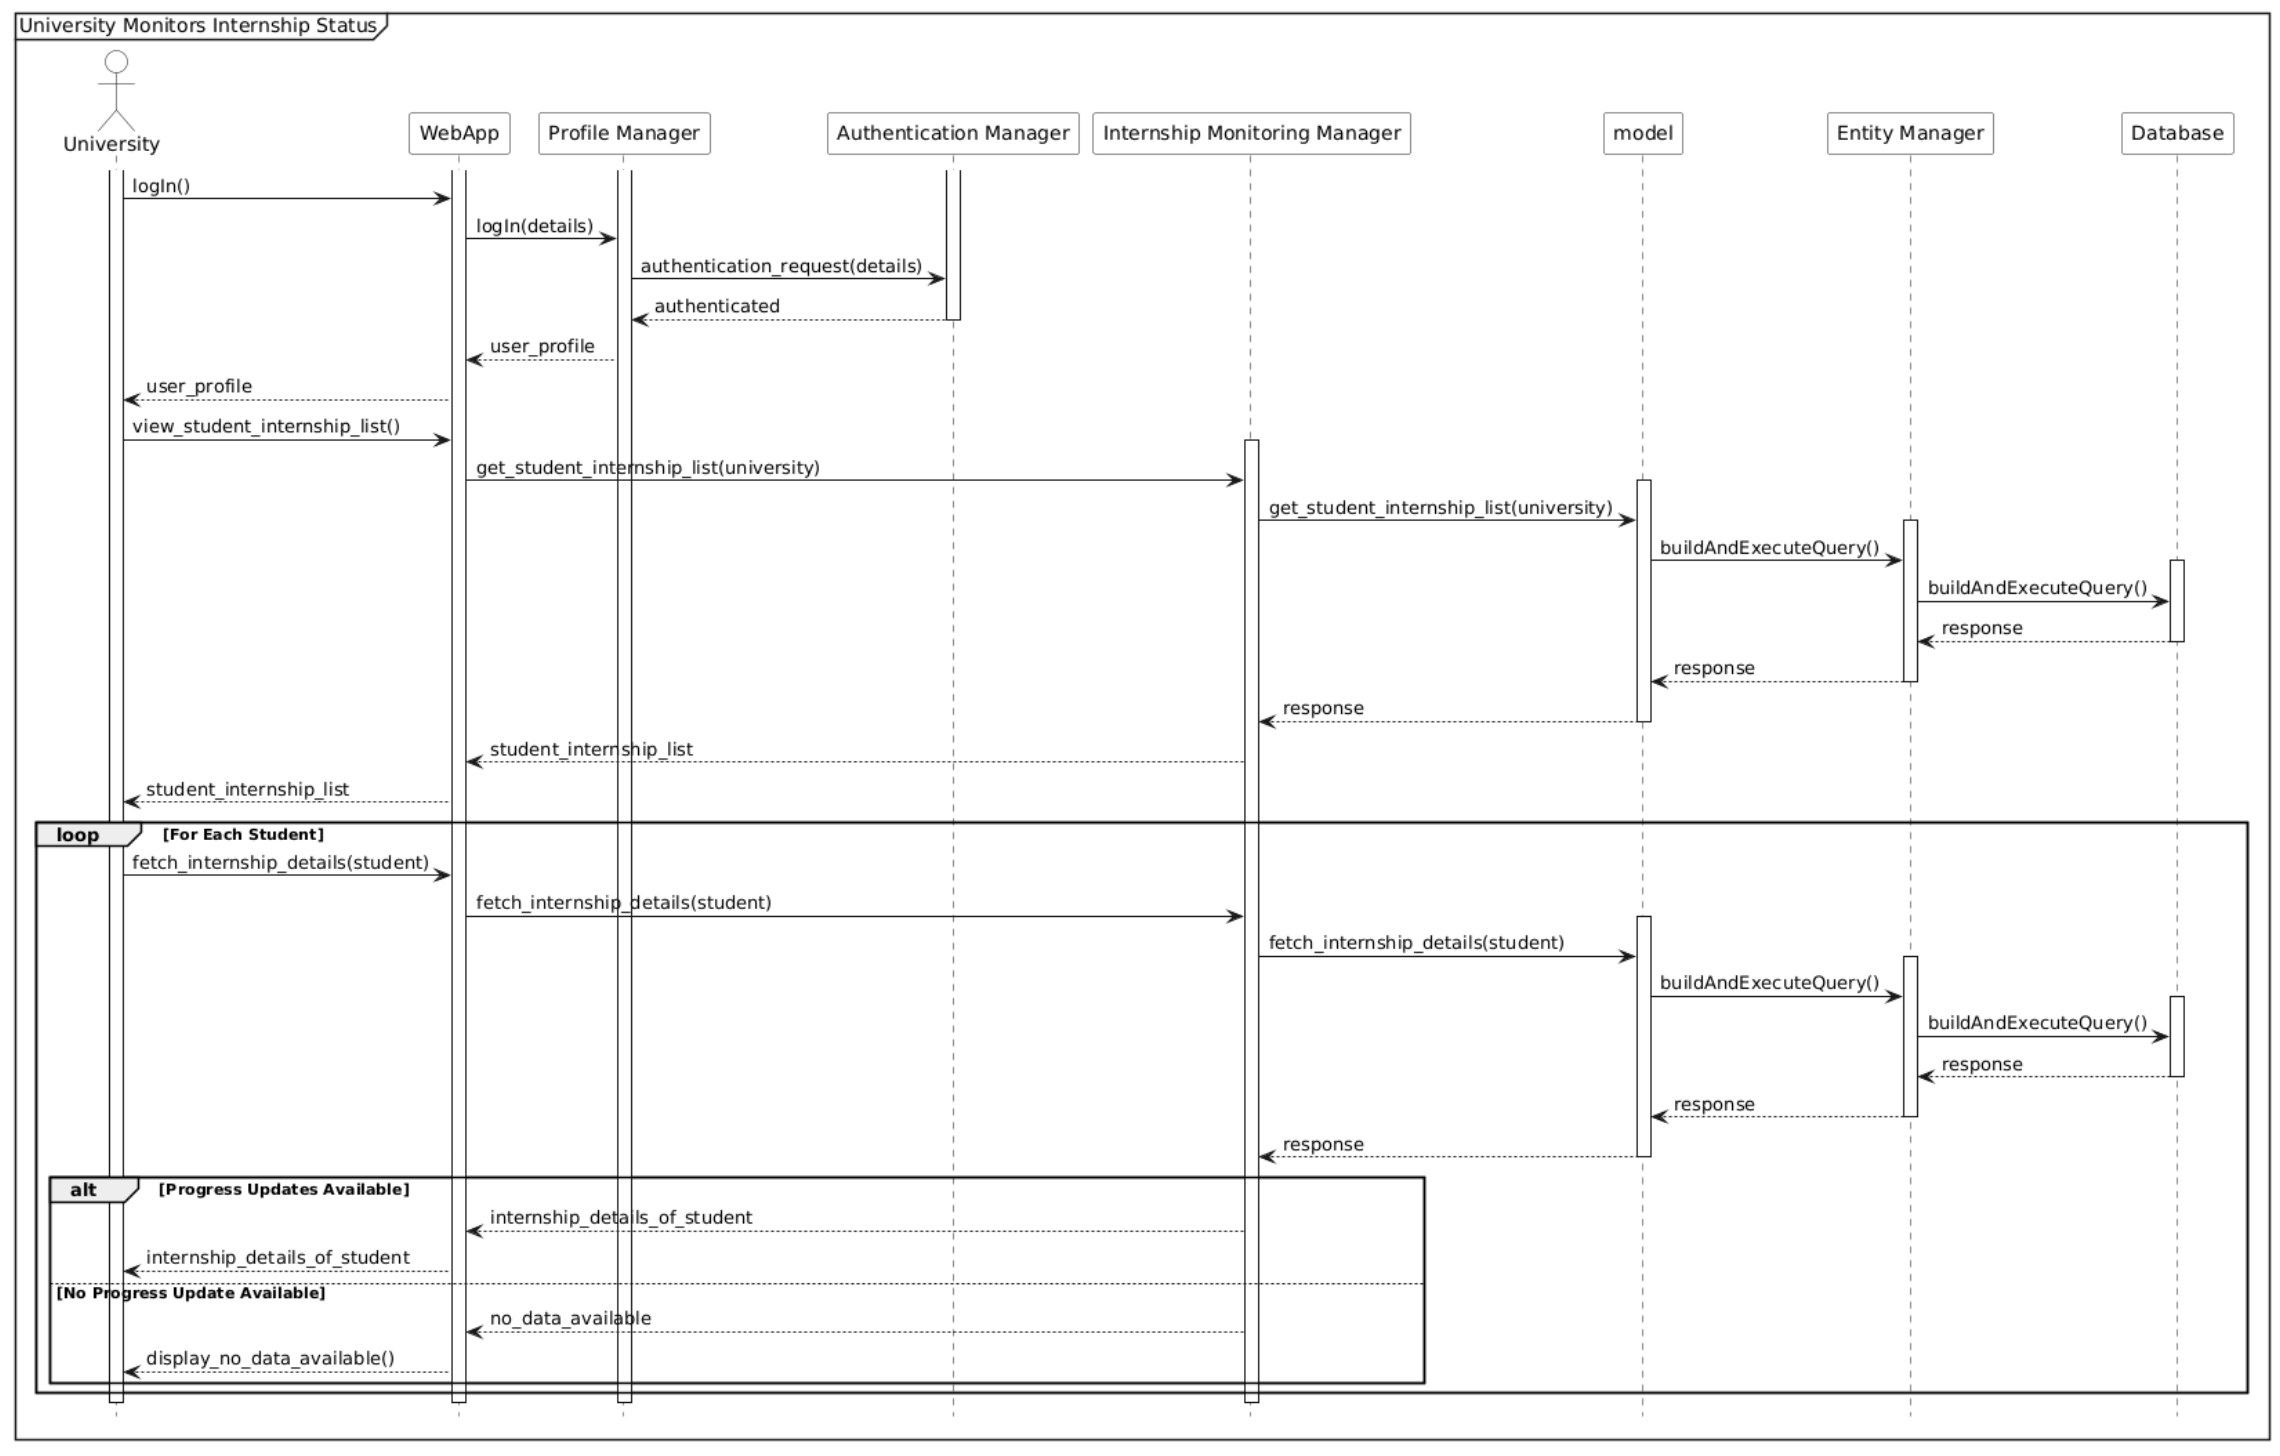
\includegraphics[width=0.8\textwidth]{Images/Uni_monitors_internship_status_sequence_diag.png}
    \caption{\label{fig:metamodel9}[UC16] Monitor Internship Status Sequence Diagram}
    \end{figure}
    \item \textbf{Handle Complaints and Issues} \\ \\
    University can login in to the S\&C web application then click on show complaints. It will fetch complaints through the Complaints Manager. If any complaints exist, university can take any decision which will be notified to the students and then mark the complaint as "Resolved" for flag for further actions required. In both the cases the complaint status and details will be updated in the database. The following diagram is the runtime sequence diagram for the Handle Complaints and Issues Sequence Diagram use case.
    \begin{figure}[H]
    \centering
    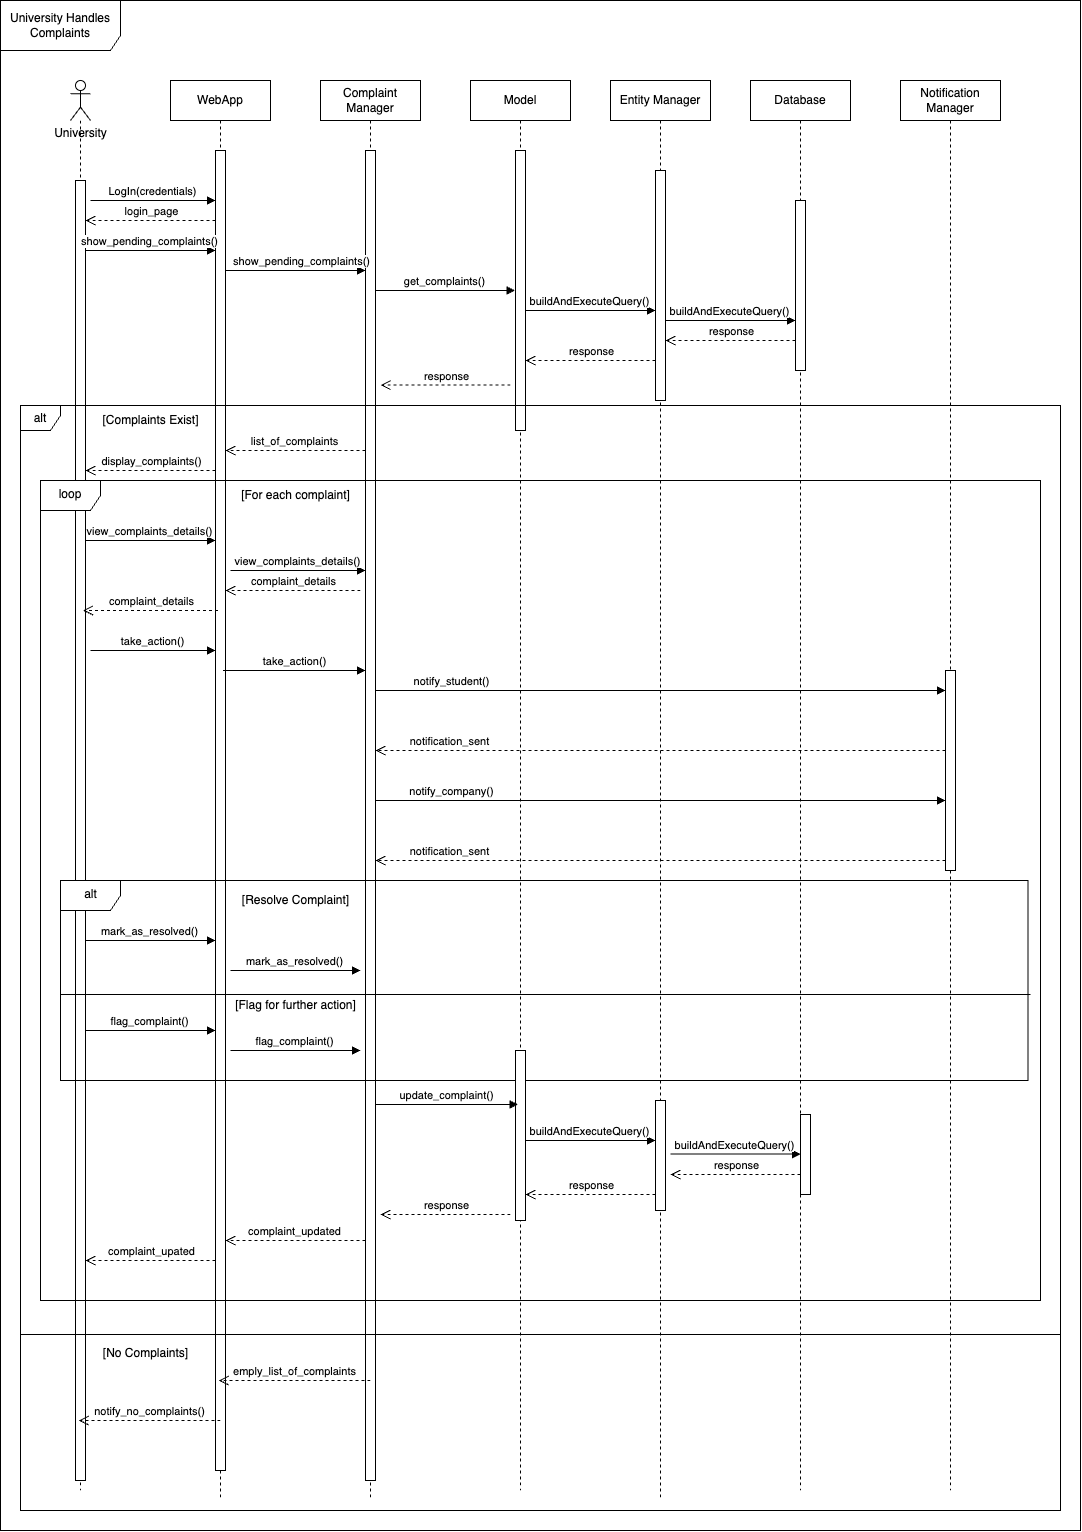
\includegraphics[width=0.8\textwidth]{Images/Uni_handles_complaints.png}
    \caption{\label{fig:metamodel9}[UC17] University Handles Complaints Sequence Diagram}
    \end{figure}
\end{itemize}

% 
\clearpage
\subsection{Component interfaces}

In this section as to represent Component interfaces we are representing API endpoints. The main focus is on the methods used, the
parameters required and on the responses.\\ 

\begin{figure}[H]
\centering
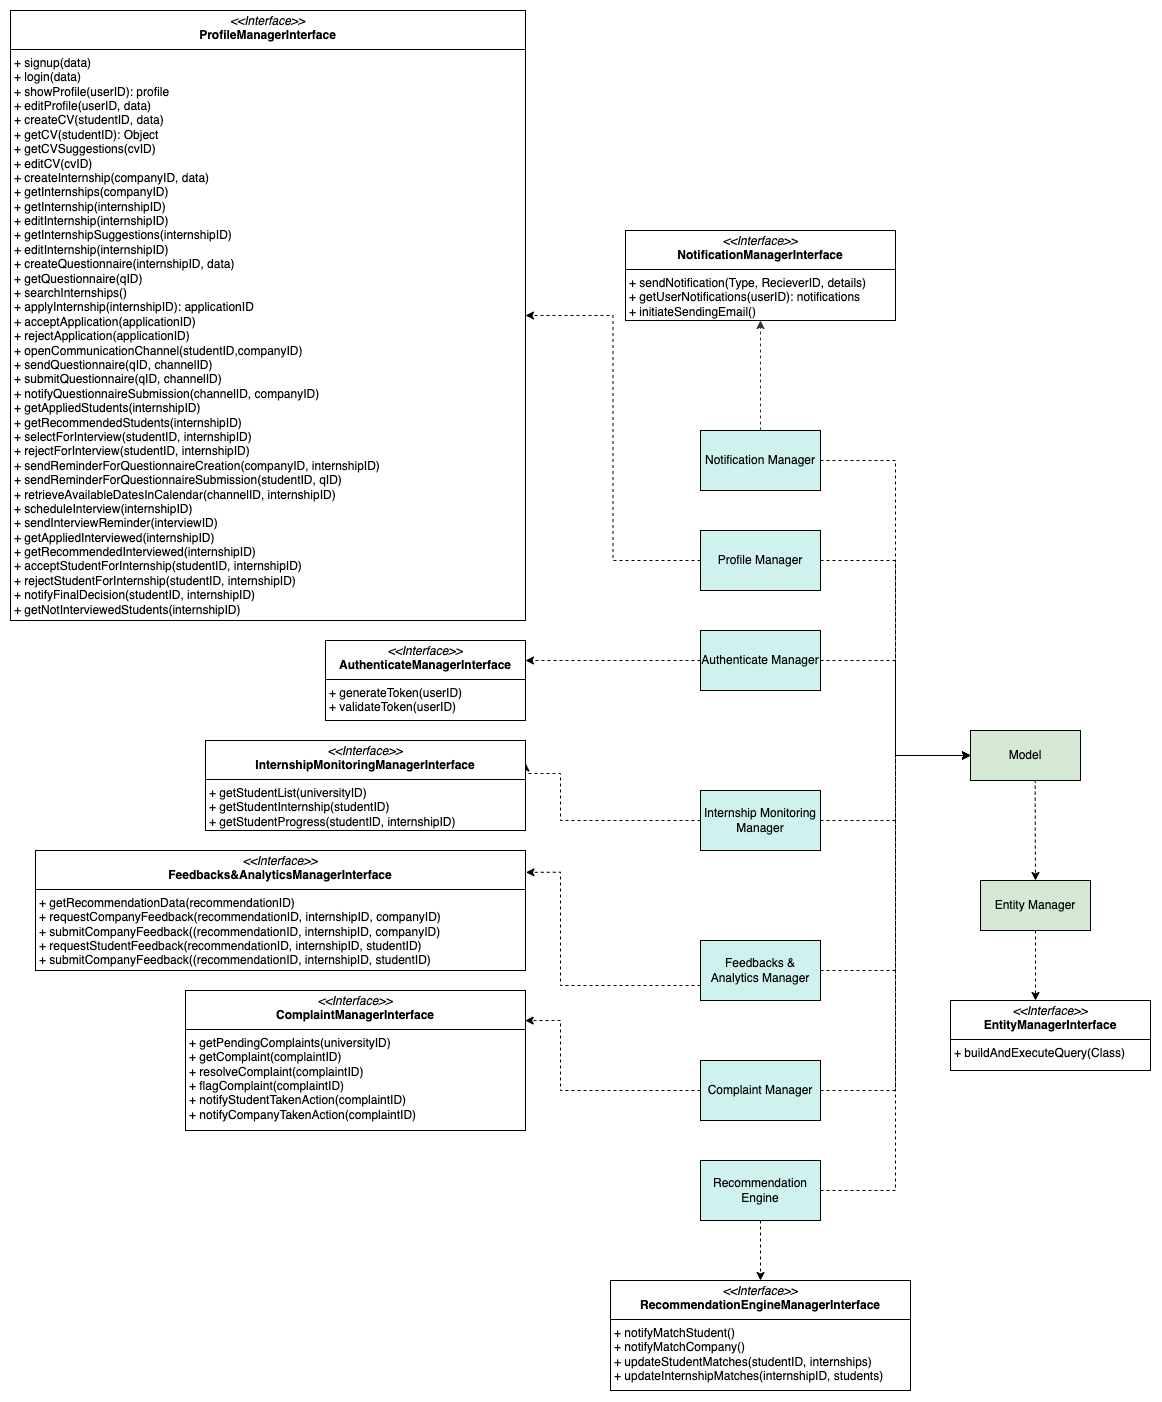
\includegraphics[width=0.8\textwidth]{Images/component_interfaces_class_diagram.png}
\caption{\label{fig:metamodel4} Component Interfaces Class Diagram}
\end{figure}

\subsubsection{API Endpoints}

\begin{itemize}
    \item \textbf{POST /api/users/signup}  
    \begin{itemize}
        \item \textbf{Description:} Registers a new user.
        \item \textbf{Request Body:} \texttt{\{ name, email, password, role, ...\}}
        \item \textbf{Response:}
        \begin{itemize}
            \item 201 Created: \texttt{\{ userId \}}
            \item 400 Bad Request: Validation errors.
        \end{itemize}
    \end{itemize}

    \item \textbf{POST /api/users/login}  
    \begin{itemize}
        \item \textbf{Description:} Logs in an existing user.
        \item \textbf{Request Body:} \texttt{\{ email, password \}}
        \item \textbf{Response:}
        \begin{itemize}
            \item 200 OK: \texttt{\{ token, userDetails \}}
            \item 401 Unauthorized: Invalid credentials.
        \end{itemize}
    \end{itemize}

    \item \textbf{GET /api/users/profile/\{userId\}}  
    \begin{itemize}
        \item \textbf{Description:} Fetches the profile of a user.
        \item \textbf{Path Parameters:} \texttt{userId}
        \item \textbf{Response:}
        \begin{itemize}
            \item 200 OK: \texttt{\{ userProfile \}}
            \item 404 Not Found: User does not exist.
        \end{itemize}
    \end{itemize}

    \item \textbf{PUT /api/users/editprofile/\{userId\}}  
    \begin{itemize}
        \item \textbf{Description:} Updates the profile of a user.
        \item \textbf{Request Body:} \texttt{\{ profileUpdates \}}
        \item \textbf{Response:}
        \begin{itemize}
            \item 200 OK: \texttt{\{ success: true \}}
            \item 400 Bad Request: Validation errors.
        \end{itemize}
    \end{itemize}

    \item \textbf{POST /api/cv/create}  
    \begin{itemize}
        \item \textbf{Description:} Creates a CV for a student.
        \item \textbf{Request Body:} \texttt{\{ studentId, cvDetails \}}
        \item \textbf{Response:}
        \begin{itemize}
            \item 201 Created: \texttt{\{ cvId \}}
            \item 400 Bad Request: Validation errors.
        \end{itemize}
    \end{itemize}
    
    \item \textbf{GET /api/cv/getcv/\{studentId\}}  
    \begin{itemize}
        \item \textbf{Description:} Retrieves the CV of a specific student.
        \item \textbf{Path Parameters:} \texttt{studentId}
        \item \textbf{Response:}
        \begin{itemize}
            \item 200 OK: \texttt{\{ cvDetails \}}
            \item 404 Not Found: No CV found for the specified student.
        \end{itemize}
    \end{itemize}

    \item \textbf{POST /api/cv/suggestions/\{studentId\}}  
    \begin{itemize}
        \item \textbf{Description:} Requests suggestions for improving a specific student's CV.
        \item \textbf{Path Parameters:} \texttt{studentId}
        \item \textbf{Request Body:} \texttt{\{ details: [...] \}}
        \item \textbf{Response:}
        \begin{itemize}
            \item 200 OK: \texttt{\{ suggestions: [...] \}}
            \item 404 Not Found: CV not found for the specified student.
            \item 400 Bad Request: Validation errors.
        \end{itemize}
    \end{itemize}

    \item \textbf{POST /api/cv/edit/\{cvId\}}  
    \begin{itemize}
        \item \textbf{Description:} Allows a student to edit an existing CV.
        \item \textbf{Path Parameters:} \texttt{cvId}
        \item \textbf{Request Body:} \texttt{\{ updatedCvDetails \}}
        \item \textbf{Response:}
        \begin{itemize}
            \item 200 OK: \texttt{\{ success: true, message: "CV updated successfully." \}}
            \item 404 Not Found: No CV found with the specified \texttt{cvId}.
            \item 400 Bad Request: Validation errors in the provided CV details.
        \end{itemize}
    \end{itemize}


    \item \textbf{POST /api/companies/internships/create/\{companyId\}}  
    \begin{itemize}
        \item \textbf{Description:} Creates a new internship posting for a specific company.
        \item \textbf{Path Parameters:} \texttt{companyId}
        \item \textbf{Request Body:} \texttt{\{ title, description, requirements \}}
        \item \textbf{Response:}
        \begin{itemize}
            \item 201 Created: \texttt{\{ internshipId \}}
            \item 400 Bad Request: Validation errors.
        \end{itemize}
    \end{itemize}
    
    \item \textbf{GET /api/companies/internships/\{companyId\}}  
    \begin{itemize}
        \item \textbf{Description:} Retrieves a list of internships for a specific company.
        \item \textbf{Path Parameters:} \texttt{companyId}
        \item \textbf{Query Parameters:} \texttt{\{ filterOptions \}}
        \item \textbf{Response:}
        \begin{itemize}
            \item 200 OK: \texttt{\{ internships: [...] \}}
            \item 401 Unauthorized: Access denied.
        \end{itemize}
    \end{itemize}

    \item \textbf{GET /api/internships/details/\{internshipId\}}  
    \begin{itemize}
        \item \textbf{Description:} Retrieves detailed information about a specific internship.
        \item \textbf{Path Parameters:} \texttt{internshipId}
        \item \textbf{Response:}
        \begin{itemize}
            \item 200 OK: \texttt{\{ internshipDetails: { ... } \}}
            \item 404 Not Found: No internship found with the specified \texttt{internshipId}.
            \item 400 Bad Request: Invalid internship ID.
        \end{itemize}
    \end{itemize}


    \item \textbf{POST /api/companies/internships/suggestions/\{companyId\}/\{internshipId\}} 
    \begin{itemize}
        \item \textbf{Description:} Requests suggestions for improving a specific internship post created by a specific company.
        \item \textbf{Path Parameters:} \texttt{companyId}, \texttt{internshipId}
        \item \textbf{Request Body:} \texttt{\{ details: [...] \}}
        \item \textbf{Response:}
        \begin{itemize}
            \item 200 OK: \texttt{\{ suggestions: [...] \}}
            \item 404 Not Found: Internship not found for the specified company.
            \item 400 Bad Request: Validation errors.
        \end{itemize}
    \end{itemize}


    \item \textbf{POST /api/internships/edit/\{internshipId\}}  
    \begin{itemize}
        \item \textbf{Description:} Allows a company to edit an existing internship posting.
        \item \textbf{Path Parameters:} \texttt{internshipId}
        \item \textbf{Request Body:} \texttt{\{ updatedInternshipDetails \}}
        \item \textbf{Response:}
        \begin{itemize}
            \item 200 OK: \texttt{\{ success: true, message: "Internship updated successfully." \}}
            \item 404 Not Found: No internship found with the specified \texttt{internshipId}.
            \item 400 Bad Request: Validation errors in the provided internship details.
        \end{itemize}
    \end{itemize}


    
    \item \textbf{POST /api/internships/questionnaire/\{internshipId\}}  
    \begin{itemize}
        \item \textbf{Description:} Creates a questionnaire for an internship.
        \item \textbf{Request Body:} \texttt{\{ questions: [...], internshipId \}}
        \item \textbf{Response:}
        \begin{itemize}
            \item 201 Created: \texttt{\{ questionnaireId \}}
            \item 400 Bad Request: Validation errors.
        \end{itemize}
    \end{itemize}
    
    \item \textbf{GET /api/internships/questionnaire/\{internshipId\}}  
    \begin{itemize}
        \item \textbf{Description:} Retrieves the questionnaire for an internship.
        \item \textbf{Path Parameters:} \texttt{internshipId}
        \item \textbf{Response:}
        \begin{itemize}
            \item 200 OK: \texttt{\{ questionnaireDetails \}}
            \item 404 Not Found: Questionnaire not found.
        \end{itemize}
    \end{itemize}

    \item \textbf{POST /api/notifications/student/matches/\{studentId\}}  
    \begin{itemize}
        \item \textbf{Description:} Sends a notification to a student about matching internships found.
        \item \textbf{Path Parameters:} studentId  
        \item \textbf{Request Body:} 
        \texttt{\{ 
            "matches": [...] 
        \}}
        \item \textbf{Response:}
        \begin{itemize}
            \item 200 OK: \texttt{\{ success: true, message: "Notification sent to student." \}}
            \item 404 Not Found: Student not found.
            \item 500 Internal Server Error: Notification sending failed.
        \end{itemize}
    \end{itemize}


    \item \textbf{POST /api/notifications/company/matches/\{companyId\}}  
    \begin{itemize}
        \item \textbf{Description:} Sends a notification to a company about matching students found for an internship.
        \item \textbf{Path Parameters:} companyId  
        \item \textbf{Request Body:} 
        \texttt{\{ 
            "matches": [...] 
        \}}
        \item \textbf{Response:}
        \begin{itemize}
            \item 200 OK: \texttt{\{ success: true, message: "Notification sent to company." \}}
            \item 404 Not Found: Company not found.
            \item 500 Internal Server Error: Notification sending failed.
        \end{itemize}
    \end{itemize}

    \item \textbf{POST /api/dashboards/student/update-matches\{studentId\}}  
    \begin{itemize}
        \item \textbf{Description:} Updates a student's dashboard with the latest matches found by the recommendation engine.
        \item \textbf{Path Parameters:} studentId  
        \item \textbf{Request Body:} 
        \texttt{\{ 
            "matches": [...] 
        \}}
        \item \textbf{Response:}
        \begin{itemize}
            \item 200 OK: \texttt{\{ success: true, message: "Dashboard updated successfully." \}}
            \item 404 Not Found: Student not found.
            \item 500 Internal Server Error: Dashboard update failed.
        \end{itemize}
    \end{itemize}

    \item \textbf{POST /api/dashboards/company/update-matches/\{companyId\}}  
    \begin{itemize}
        \item \textbf{Description:} Updates a company's dashboard with the latest matches found by the recommendation engine.
        \item \textbf{Path Parameters:} companyId  
        \item \textbf{Request Body:} 
        \texttt{\{ 
            "matches": [...] 
        \}}
        \item \textbf{Response:}
        \begin{itemize}
            \item 200 OK: \texttt{\{ success: true, message: "Dashboard updated successfully." \}}
            \item 404 Not Found: Company not found.
            \item 500 Internal Server Error: Dashboard update failed.
        \end{itemize}
    \end{itemize}

    \item \textbf{GET /api/internships/search}  
    \begin{itemize}
        \item \textbf{Description:} Allows a student to search for internships based on specified criterias.
        \item \textbf{Request Body:} A JSON object containing the search criteria.
        \item \textbf{Response:}
        \begin{itemize}
            \item 200 OK: \texttt{\{ internships: [...] \}}
            \begin{itemize}
                \item Returns a list of internships that match the given criteria.
            \end{itemize}
            \item 400 Bad Request: Validation errors in the provided criteria.
            \item 401 Unauthorized: User is not authenticated.
        \end{itemize}
    \end{itemize}


    \item \textbf{POST /api/internships/apply/\{internshipId\}}  
    \begin{itemize}
        \item \textbf{Description:} Allows a student to apply to a specific internship.
        \item \textbf{Request Body:} A JSON object containing the application details.
        \item \textbf{Path Parameters:}  
        \begin{itemize}
            \item \texttt{internshipId}: The ID of the internship the student is applying to.
        \end{itemize}
        \item \textbf{Response:}
        \begin{itemize}
            \item 200 OK: \texttt{\{ success: true, message: "Application submitted successfully." \}}
            \item 400 Bad Request: Validation errors in the application details.
            \item 401 Unauthorized: User is not authenticated.
            \item 404 Not Found: Internship not found.
        \end{itemize}
    \end{itemize}


    \item \textbf{POST /api/internships/applications/accept/\{internshipId\}/\{applicationId\}}  
    \begin{itemize}
        \item \textbf{Description:} Allows a company to accept a student's application for a specific internship.
        \item \textbf{Path Parameters:}  
        \begin{itemize}
            \item \texttt{internshipId}: The ID of the internship the application belongs to.
            \item \texttt{applicationId}: The ID of the student's application.
        \end{itemize}
        \item \textbf{Response:}
        \begin{itemize}
            \item 200 OK: \texttt{\{ success: true, message: "Application accepted successfully." \}}
            \item 400 Bad Request: Validation errors or missing data.
            \item 401 Unauthorized: User is not authenticated or authorized.
            \item 404 Not Found: Internship or application not found.
        \end{itemize}
    \end{itemize}

    \item \textbf{POST /api/internships/applications/reject/\{internshipId\}/\{applicationId\}}  
    \begin{itemize}
        \item \textbf{Description:} Allows a company to reject a student's application for a specific internship.
        \item \textbf{Path Parameters:} internshipId, applicationId  
        \item \textbf{Response:}
        \begin{itemize}
            \item 200 OK: \texttt{\{ success: true, message: "Application rejected successfully." \}}
            \item 400 Bad Request: Validation errors or missing data.
            \item 401 Unauthorized: User is not authenticated or authorized.
            \item 404 Not Found: Internship or application not found.
        \end{itemize}
    \end{itemize}


    \item \textbf{POST /api/communication/open/\{studentId\}/\{companyId\}}  
    \begin{itemize}
        \item \textbf{Description:} Opens a communication channel between a student and a company during the selection process.
        \item \textbf{Path Parameters:} studentId, companyId  
        \item \textbf{Response:}
        \begin{itemize}
            \item 200 OK: \texttt{\{ success: true, message: "Communication channel opened successfully." \}}
            \item 400 Bad Request: Validation errors in the request.
            \item 401 Unauthorized: User is not authenticated.
        \end{itemize}
    \end{itemize}


    \item \textbf{POST /api/questionnaire/send/\{qId\}/\{studentId\}/\{internshipId\}/\{channelId\}}  
    \begin{itemize}
        \item \textbf{Description:} Sends a questionnaire from the company to a student as part of the selection process.
        \item \textbf{Path Parameters:} studentId, internshipId, channelId, qId  
        \item \textbf{Request Body:} 
        \texttt{\{ 
            "questions": ["string", "string", ...]
        \}}
        \item \textbf{Response:}
        \begin{itemize}
            \item 200 OK: \texttt{\{ success: true, message: "Questionnaire sent successfully." \}}
            \item 404 Not Found: Internship or student not found.
            \item 400 Bad Request: Validation errors in the request body.
        \end{itemize}
    \end{itemize}

    \item \textbf{POST /api/questionnaire/submit//\{qId\}\{studentId\}/\{internshipId\}/\{channelId\}}  
    \begin{itemize}
        \item \textbf{Description:} Allows a student to submit answers to a received questionnaire.
        \item \textbf{Path Parameters:} studentId, internshipId, channelId, qId 
        \item \textbf{Request Body:} 
        \texttt{\{ 
            "answers": ["string", "string", ...] 
        \}}
        \item \textbf{Response:}
        \begin{itemize}
            \item 200 OK: \texttt{\{ success: true, message: "Answers submitted successfully." \}}
            \item 404 Not Found: Questionnaire not found.
            \item 400 Bad Request: Validation errors in the answers.
        \end{itemize}
    \end{itemize}

    \item \textbf{POST /api/questionnaire/notify/\{channelId\}/\{companyId\}/\{internshipId\}}  
    \begin{itemize}
        \item \textbf{Description:} Notifies the company when a questionnaire has been submitted by the student.
        \item \textbf{Path Parameters:} channelId, companyId, internshipId  
        \item \textbf{Response:}
        \begin{itemize}
            \item 200 OK: \texttt{\{ success: true, message: "Notification sent successfully." \}}
            \item 500 Internal Server Error: Failed to send the notification.
        \end{itemize}
    \end{itemize}

    \item \textbf{GET /api/internships/applied-students/\{internshipId\}}  
    \begin{itemize}
        \item \textbf{Description:} Retrieves a list of students who applied for a specific internship.
        \item \textbf{Path Parameters:} \texttt{internshipId}
        \item \textbf{Response:}
        \begin{itemize}
            \item 200 OK: \texttt{\{ students: [...] \}}
            \item 404 Not Found: No internship found with the specified \texttt{internshipId}, or no students applied.
            \item 400 Bad Request: Invalid internship ID.
        \end{itemize}
    \end{itemize}


    \item \textbf{GET /api/internships/recommended-students/\{internshipId\}}  
    \begin{itemize}
        \item \textbf{Description:} Retrieves a list of students recommended by the system for a specific internship.
        \item \textbf{Path Parameters:} \texttt{internshipId}
        \item \textbf{Response:}
        \begin{itemize}
            \item 200 OK: \texttt{\{ recommendedStudents: [...] \}}
            \item 404 Not Found: No internship found with the specified \texttt{internshipId}, or no recommended students available.
            \item 400 Bad Request: Invalid internship ID.
        \end{itemize}
    \end{itemize}



    \item \textbf{POST /api/interviews/select/\{studentId\}/\{internshipId\}}  
    \begin{itemize}
        \item \textbf{Description:} Adds a student to the interview shortlist for a specific internship.
        \item \textbf{Path Parameters:} studentId, internshipId  
        \item \textbf{Response:}
        \begin{itemize}
            \item 200 OK: \texttt{\{ success: true, message: "Student added to interview shortlist." \}}
            \item 404 Not Found: Internship or student not found.
            \item 400 Bad Request: Validation errors in the request.
        \end{itemize}
    \end{itemize}



    \item \textbf{POST /api/interviews/reject/\{studentId\}/\{internshipId\}}  
    \begin{itemize}
        \item \textbf{Description:} Rejects a student for a specific internship and removes them from the selection process.
        \item \textbf{Path Parameters:} studentId, internshipId  
        \item \textbf{Response:}
        \begin{itemize}
            \item 200 OK: \texttt{\{ success: true, message: "Student rejected successfully." \}}
            \item 404 Not Found: Internship or student not found.
            \item 400 Bad Request: Validation errors in the request.
        \end{itemize}
    \end{itemize}

    \item \textbf{POST /api/questionnaire/reminder/\{studentId\}/\{internshipId\}}  
    \begin{itemize}
        \item \textbf{Description:} Sends a reminder to the student about an incomplete questionnaire.
        \item \textbf{Path Parameters:} studentId, internshipId  
        \item \textbf{Response:}
        \begin{itemize}
            \item 200 OK: \texttt{\{ success: true, message: "Reminder sent successfully." \}}
            \item 404 Not Found: Questionnaire not found.
            \item 500 Internal Server Error: Failed to send the reminder.
        \end{itemize}
    \end{itemize}

    \item \textbf{POST /api/questionnaire/reminder/\{studentId\}/\{qId\}}  
    \begin{itemize}
        \item \textbf{Description:} Sends a reminder to a student to complete and submit a specific questionnaire.
        \item \textbf{Path Parameters:} \texttt{studentId}, \texttt{qId}
        \item \textbf{Response:}
        \begin{itemize}
            \item 200 OK: \texttt{\{ success: true, message: "Reminder sent successfully." \}}
            \item 404 Not Found: Student or questionnaire not found with the specified IDs.
            \item 400 Bad Request: Invalid student ID or questionnaire ID.
            \item 500 Internal Server Error: Failed to send the reminder.
        \end{itemize}
    \end{itemize}


    \item \textbf{GET /api/interviews/calendar/\{internshipId\}/\{channelId\}}  
    \begin{itemize}
        \item \textbf{Description:} Retrieves available dates and times for scheduling an interview.
        \item \textbf{Path Parameters:} internshipId, channelId
        \item \textbf{Response:}
        \begin{itemize}
            \item 200 OK: \texttt{\{ availableDates: [ "YYYY-MM-DD HH:mm", ... ] \}}
            \item 400 Bad Request: Invalid internship ID or unavailable calendar data.
            \item 401 Unauthorized: User is not authenticated.
        \end{itemize}
    \end{itemize}

    \item \textbf{POST /api/interviews/schedule/\{internshipId\}}  
    \begin{itemize}
        \item \textbf{Description:} Schedules an interview for a specific internship by providing date, time, and meeting link details in the student's and company's dashboard.
        \item \textbf{Path Parameters:} 
        \begin{itemize}
            \item \texttt{internshipId}: The ID of the internship for which the interview is being scheduled.
        \end{itemize}
        \item \textbf{Request Body:} 
        \texttt{\{ 
            "date": "YYYY-MM-DD", 
            "time": "HH:mm", 
            "meetingLink": "string" 
        \}}
        \item \textbf{Response:}
        \begin{itemize}
            \item 200 OK: \texttt{\{ success: true, message: "Interview scheduled successfully." \}}
            \item 400 Bad Request: Invalid date, time, or missing meeting link.
            \item 404 Not Found: Internship not found.
            \item 401 Unauthorized: User is not authenticated.
        \end{itemize}
    \end{itemize}


    \item \textbf{POST /api/interviews/notify/\{interviewId\}}  
    \begin{itemize}
        \item \textbf{Description:} Sends notifications to the student and the company about the scheduled interview.
        \item \textbf{Path Parameters:} interviewId
        \item \textbf{Request Body:} 
        \texttt{\{ 
            "message": "string"
        \}}
        \item \textbf{Response:}
        \begin{itemize}
            \item 200 OK: \texttt{\{ success: true, message: "Notifications sent successfully." \}}
            \item 404 Not Found: Interview ID not found.
            \item 500 Internal Server Error: Failed to send notifications.
        \end{itemize}
    \end{itemize}


    \item \textbf{POST /api/interviews/reminder/\{interviewId\}}  
    \begin{itemize}
        \item \textbf{Description:} Sends reminders to both the student and company before the interview.
        \item \textbf{Path Parameters:} 
        \begin{itemize}
            \item \texttt{interviewId}: The ID of the interview for which reminders will be sent.
        \end{itemize}
        \item \textbf{Response:}
        \begin{itemize}
            \item 200 OK: \texttt{\{ success: true, message: "Reminders sent successfully." \}}
            \item 404 Not Found: Interview ID not found.
            \item 500 Internal Server Error: Failed to send reminders.
        \end{itemize}
    \end{itemize}

    \item \textbf{GET /api/internships/interviewed-applied-students/\{internshipId\}}  
    \begin{itemize}
        \item \textbf{Description:} Retrieves a list of students who were interviewed and had applied for a specific internship.
        \item \textbf{Path Parameters:} internshipId  
        \item \textbf{Response:}
        \begin{itemize}
            \item 200 OK: \texttt{\{ students: [...] \}}
            \item 404 Not Found: Internship not found.
            \item 400 Bad Request: Invalid internship ID.
        \end{itemize}
    \end{itemize}

    \item \textbf{GET /api/internships/interviewed-recommended-students/\{internshipId\}}  
    \begin{itemize}
        \item \textbf{Description:} Retrieves a list of students who were interviewed based on the system's recommendations for a specific internship.
        \item \textbf{Path Parameters:} internshipId  
        \item \textbf{Response:}
        \begin{itemize}
            \item 200 OK: \texttt{\{ students: [...] \}}
            \item 404 Not Found: Internship not found.
            \item 400 Bad Request: Invalid internship ID.
        \end{itemize}
    \end{itemize}

    \item \textbf{POST /api/internships/accept/\{internshipId\}/\{studentId\}}  
    \begin{itemize}
        \item \textbf{Description:} Accepts a student for a specific internship and notifies them.
        \item \textbf{Path Parameters:} internshipId, studentId  
        \item \textbf{Response:}
        \begin{itemize}
            \item 200 OK: \texttt{\{ success: true, message: "Student accepted and notified." \}}
            \item 404 Not Found: Internship or student not found.
            \item 400 Bad Request: Invalid parameters.
        \end{itemize}
    \end{itemize}

    \item \textbf{POST /api/internships/reject/\{internshipId\}/\{studentId\}}  
    \begin{itemize}
        \item \textbf{Description:} Rejects a student for a specific internship and notifies them.
        \item \textbf{Path Parameters:} internshipId, studentId  
        \item \textbf{Response:}
        \begin{itemize}
            \item 200 OK: \texttt{\{ success: true, message: "Student rejected and notified." \}}
            \item 404 Not Found: Internship or student not found.
            \item 400 Bad Request: Invalid parameters.
        \end{itemize}
    \end{itemize}

    \item \textbf{POST /api/internships/notify/\{internshipId\}/\{studentId\}}  
    \begin{itemize}
        \item \textbf{Description:} notifies the student of the final decision for a specific student in the context of an internship (either accept or reject).
        \item \textbf{Path Parameters:} internshipId, studentId  
        \item \textbf{Request Body:} 
        \texttt{\{ 
            "message": "string"
        \}}
        \item \textbf{Response:}
        \begin{itemize}
            \item 200 OK: \texttt{\{ success: true, message: "Final decision notified." \}}
            \item 404 Not Found: Internship or student not found.
            \item 400 Bad Request: Invalid decision or parameters.
        \end{itemize}
    \end{itemize}

    \item \textbf{GET /api/internships/no-interviewed-students/\{internshipId\}}  
    \begin{itemize}
        \item \textbf{Description:} Checks if there are no interviewed students left for finalization in a specific internship.
        \item \textbf{Path Parameters:} internshipId  
        \item \textbf{Response:}
        \begin{itemize}
            \item 200 OK: \texttt{\{ noStudents: true | false \}}
            \item 404 Not Found: Internship not found.
            \item 400 Bad Request: Invalid internship ID.
        \end{itemize}
    \end{itemize}


    \item \textbf{GET /api/recommendations/data/\{recommendationId\}}  
    \begin{itemize}
        \item \textbf{Description:} Retrieves detailed data about a specific recommendation.
        \item \textbf{Path Parameters:} recommendationId  
        \item \textbf{Response:}
        \begin{itemize}
            \item 200 OK: \texttt{\{ recommendationData: { ... } \}}
            \item 404 Not Found: Recommendation not found.
            \item 400 Bad Request: Invalid recommendation ID.
        \end{itemize}
    \end{itemize}

    \item \textbf{POST /api/feedback/request/company/\{internshipId\}/\{companyId\}/\{recommendationId\}}  
    \begin{itemize}
        \item \textbf{Description:} Sends a request to the company for feedback on a specific recommendation.
        \item \textbf{Path Parameters:} internshipId, companyId, recommendationId  
        \item \textbf{Response:}
        \begin{itemize}
            \item 200 OK: \texttt{\{ success: true, message: "Feedback request sent to the company." \}}
            \item 404 Not Found: Internship, company, or recommendation not found.
            \item 400 Bad Request: Invalid recommendation ID.
        \end{itemize}
    \end{itemize}

    \item \textbf{POST /api/feedback/submit/company/\{internshipId\}/\{companyId\}/\{recommendationId\}}  
    \begin{itemize}
        \item \textbf{Description:} Allows a company to submit feedback on a specific recommendation.
        \item \textbf{Path Parameters:} internshipId, companyId, recommendationId  
        \item \textbf{Request Body:} 
        \texttt{\{ 
            "feedback": Object
        \}}
        \item \textbf{Response:}
        \begin{itemize}
            \item 200 OK: \texttt{\{ success: true, message: "Feedback submitted successfully." \}}
            \item 404 Not Found: Internship, company, or recommendation not found.
            \item 400 Bad Request: Validation errors in the feedback.
        \end{itemize}
    \end{itemize}

    \item \textbf{POST /api/feedback/request/student/\{internshipId\}/\{studentId\}/\{recommendationId\}}  
    \begin{itemize}
        \item \textbf{Description:} Sends a request to a student for feedback on a specific recommendation.
        \item \textbf{Path Parameters:} internshipId, studentId, recommendationId  
        \item \textbf{Response:}
        \begin{itemize}
            \item 200 OK: \texttt{\{ success: true, message: "Feedback request sent to the student." \}}
            \item 404 Not Found: Internship, student, or recommendation not found.
            \item 400 Bad Request: Invalid recommendation ID.
        \end{itemize}
    \end{itemize}


    \item \textbf{POST /api/feedback/submit/student/\{internshipId\}/\{studentId\}/\{recommendationId\}}  
    \begin{itemize}
        \item \textbf{Description:} Allows a student to submit feedback on a specific recommendation.
        \item \textbf{Path Parameters:} internshipId, studentId, recommendationId  
        \item \textbf{Request Body:} 
        \texttt{\{ 
            "feedback": Object
        \}}
        \item \textbf{Response:}
        \begin{itemize}
            \item 200 OK: \texttt{\{ success: true, message: "Feedback submitted successfully." \}}
            \item 404 Not Found: Internship, student, or recommendation not found.
            \item 400 Bad Request: Validation errors in the feedback.
        \end{itemize}
    \end{itemize}

    \item \textbf{POST /api/feedback/save/\{recommendationId\}}  
    \begin{itemize}
        \item \textbf{Description:} Saves feedback provided by a student or company for a specific recommendation to the database.
        \item \textbf{Path Parameters:} recommendationId  
        \item \textbf{Request Body:} 
        \texttt{\{ 
            "feedback": Object
        \}}
        \item \textbf{Response:}
        \begin{itemize}
            \item 200 OK: \texttt{\{ success: true, message: "Feedback saved successfully." \}}
            \item 404 Not Found: Recommendation not found.
            \item 400 Bad Request: Validation errors in the feedback.
        \end{itemize}
    \end{itemize}

    \item \textbf{GET /api/internships/student-list/university/\{universityId\}}  
    \begin{itemize}
        \item \textbf{Description:} Retrieves a list of students and their internships associated with a specific university.
        \item \textbf{Path Parameters:} universityId  
        \item \textbf{Response:}
        \begin{itemize}
            \item 200 OK: \texttt{\{ students: [...] \}}
            \item 404 Not Found: University not found or no students associated.
            \item 400 Bad Request: Invalid university ID.
        \end{itemize}
    \end{itemize}

    \item \textbf{GET /api/internships/details/student/\{studentId\}}  
    \begin{itemize}
        \item \textbf{Description:} Retrieves detailed internship information for a specific student.
        \item \textbf{Path Parameters:} studentId  
        \item \textbf{Response:}
        \begin{itemize}
            \item 200 OK: \texttt{\{ internshipDetails: { ... } \}}
            \item 404 Not Found: Student or internship details not found.
            \item 400 Bad Request: Invalid student ID.
        \end{itemize}
    \end{itemize}

    \item \textbf{GET /api/internships/progress/student/\{studentId\}/\{internshipId\}}  
    \begin{itemize}
        \item \textbf{Description:} Retrieves progress updates for a student's internship.
        \item \textbf{Path Parameters:} studentId, internshipId
        \item \textbf{Response:}
        \begin{itemize}
            \item 200 OK: \texttt{\{ progressUpdates: [...] \}}
            \item 404 Not Found: No progress updates available for the student.
            \item 400 Bad Request: Invalid student ID.
        \end{itemize}
    \end{itemize}
    
    \item \textbf{GET /api/complaints/pending/university/\{universityId\}}  
    \begin{itemize}
        \item \textbf{Description:} Retrieves a list of pending complaints for the university.
        \item \textbf{Path Parameters:} universityId  
        \item \textbf{Response:}
        \begin{itemize}
            \item 200 OK: \texttt{\{ complaints: [...] \}}
            \item 404 Not Found: University or complaints not found.
            \item 400 Bad Request: Invalid university ID.
        \end{itemize}
    \end{itemize}

    \item \textbf{GET /api/complaints/details/\{complaintId\}}  
    \begin{itemize}
        \item \textbf{Description:} Retrieves the details of a specific complaint.
        \item \textbf{Path Parameters:} complaintId  
        \item \textbf{Response:}
        \begin{itemize}
            \item 200 OK: \texttt{\{ complaintDetails: { ... } \}}
            \item 404 Not Found: Complaint not found.
            \item 400 Bad Request: Invalid complaint ID.
        \end{itemize}
    \end{itemize}

    \item \textbf{POST /api/notifications/student/complaint/\{studentId\}/\{complaintId\}}  
    \begin{itemize}
        \item \textbf{Description:} Sends a notification to a student regarding the action taken on their complaint.
        \item \textbf{Path Parameters:} studentId, complaintId  
        \item \textbf{Response:}
        \begin{itemize}
            \item 200 OK: \texttt{\{ success: true, message: "Notification sent to student." \}}
            \item 404 Not Found: Student or complaint not found.
            \item 500 Internal Server Error: Failed to send notification.
        \end{itemize}
    \end{itemize}


    \item \textbf{POST /api/notifications/company/complaint/\{companyId\}/\{complaintId\}}  
    \begin{itemize}
        \item \textbf{Description:} Sends a notification to a company regarding the action taken on a complaint involving them.
        \item \textbf{Path Parameters:} companyId, complaintId  
        \item \textbf{Response:}
        \begin{itemize}
            \item 200 OK: \texttt{\{ success: true, message: "Notification sent to company." \}}
            \item 404 Not Found: Company or complaint not found.
            \item 500 Internal Server Error: Failed to send notification.
        \end{itemize}
    \end{itemize}

    \item \textbf{POST /api/complaints/resolve/\{complaintId\}}  
    \begin{itemize}
        \item \textbf{Description:} Marks a specific complaint as resolved.
        \item \textbf{Path Parameters:} complaintId  
        \item \textbf{Response:}
        \begin{itemize}
            \item 200 OK: \texttt{\{ success: true, message: "Complaint marked as resolved." \}}
            \item 404 Not Found: Complaint not found.
            \item 400 Bad Request: Invalid complaint ID.
        \end{itemize}
    \end{itemize}

    \item \textbf{POST /api/complaints/flag/\{complaintId\}}  
    \begin{itemize}
        \item \textbf{Description:} Flags a specific complaint for further action or investigation.
        \item \textbf{Path Parameters:} complaintId  
        \item \textbf{Response:}
        \begin{itemize}
            \item 200 OK: \texttt{\{ success: true, message: "Complaint flagged for further action." \}}
            \item 404 Not Found: Complaint not found.
            \item 400 Bad Request: Invalid complaint ID.
        \end{itemize}
    \end{itemize}

    \item \textbf{GET /api/notifications/\{userId\}}  
    \begin{itemize}
        \item \textbf{Description:} Retrieves notifications for a user.
        \item \textbf{Path Parameters:} \texttt{userId}
        \item \textbf{Response:}
        \begin{itemize}
            \item 200 OK: \texttt{\{ notifications: [...] \}}
            \item 401 Unauthorized: Access denied.
        \end{itemize}
    \end{itemize}

\end{itemize}
\subsection{Selected Architectural Styles and Patterns}

\subsubsection{Three-Tier Architecture}
The Three-Tier architecture divides the system into three logical layers: 
\begin{itemize}
    \item \textbf{Presentation Tier (Web Server):} This layer provides the user interface, typically through web pages or web applications. It is implemented using technologies like HTML, CSS, and JavaScript. This tier allows interaction between the user and the system.
    \item \textbf{Business Logic Tier (Application Server):} This layer acts as the intermediary, processing and implementing the business logic. It ensures the rules and workflows of the system are correctly executed. It is often responsible for making decisions and handling API requests.
    \item \textbf{Data Storage Tier (Database Server):} This is the backend layer responsible for managing and storing data. It runs on a Database Management System (DBMS), ensuring data persistence and security.
\end{itemize}
The Three-Tier architecture offers modularization, scalability, and separation of concerns, which simplifies maintenance and enhances control and security in the system.

\subsubsection{Model-View-Controller (MVC) Pattern}
The Model-View-Controller (MVC) pattern is adopted for its modular and maintainable software architecture. It is particularly well-suited for web applications:
\begin{itemize}
    \item \textbf{Model:} Manages the data, application logic, and rules of the system. It encapsulates the core functionality and ensures consistency in data handling.
    \item \textbf{View:} Represents the data visually to the users, such as charts, tables, or forms. Multiple views can exist for the same data, catering to different user needs.
    \item \textbf{Controller:} Acts as the intermediary between the Model and the View. It processes user inputs, communicates with the Model to fetch or manipulate data, and updates the View accordingly.
\end{itemize}
This pattern provides strong decoupling between the components, enhancing reliability, reusability, and clarity of the codebase. The distributed nature of this pattern supports scalable applications by efficiently handling user interfaces and data processing.

\subsubsection{RESTful APIs}
RESTful APIs (Representational State Transfer) are implemented to ensure seamless communication between the client and server. These APIs:
\begin{itemize}
    \item Use standard HTTP methods: GET, POST, PUT, DELETE, etc., for data exchange.
    \item Are stateless, ensuring each request is self-contained and independent of previous ones.
\end{itemize}
RESTful APIs are simple to implement, lightweight, and reduce server load, making them an ideal choice for scalable systems requiring smooth communication and data exchange.

\subsubsection{Cloud Hosted}
The S\&W is hosted on cloud and used third party cloud service providers for to manage and deliver services and applications. Some advantages of cloud deployment other than the already mentioned are as follows:
\begin{itemize}
    \item \textbf{High Availability:} Cloud providers offer uptime guarantees and data is often replicated across multiple data centers to ensure availability.
    \item \textbf{Security:} Cloud providers often implement strict security policies and invest heavily in infrastructure to protect data.
\end{itemize}
% \begin{itemize}
%     \item \textbf{High Availability: Cloud providers offer uptime guarantees and data is often replicated across multiple data centers to ensure availability.
%     \item \textbf{Security:} Cloud providers often implement strict security policies and invest heavily in infrastructure to protect data.
% \end{itemize}



\subsection{Other Design Decisions}

\subsubsection{Token-Based Authentication and Authorization}
The system employs a token-based authentication and authorization mechanism to secure access and maintain user sessions. Key features include:
\begin{itemize}
    \item \textbf{Token Generation:} Upon login, the server generates a unique token, such as a JWT (JSON Web Token), which is shared with the client.
    \item \textbf{Token Usage:} The token must be included in the header of every subsequent request requiring authentication or authorization.
    \item \textbf{Security Features:} Tokens are used for secure operations, such as identifying users, validating their roles, and safely sending sensitive data like email invitations.
\end{itemize}
This approach enhances security by ensuring only authenticated users can access restricted resources, while the stateless nature of tokens reduces the load on the server.

\subsubsection{Relational Database}
The system uses relational database for storing and querying of data. In relational database data is stored in a structured format using tables (called relations). This structure allows for easy querying, retrieval, and manipulation of data using a specialized query language, most commonly SQL. There are several upsides of using relational database, some of which are as follows:
\begin{itemize}
\item \textbf{Structured Data Storage:} Data is stored in a highly organized and logical manner, which makes it easy to access, manage, and update.
\item \textbf{Scalability:} Relational databases can handle large volumes of data and can scale horizontally or vertically to accommodate more records or users.
\item \textbf{Flexible Queries:} It provides powerful querying capabilities, allowing retrieval and manipulation of data in complex ways. 

\end{itemize}





